\documentclass[
    a5paper,
    pagesize,
    11pt,
    bibtotoc,
    normalheadings,
    twoside,
    openany,
    chapterprefix,
    DIV=9
]{scrbook}

\usepackage[utf8]{inputenc}
\usepackage{tocloft}
\usepackage{mathtools}
\usepackage{amsfonts}
\usepackage{enumitem}
\usepackage{amsmath}
\usepackage{amsthm}
\usepackage{amssymb}
\usepackage[hmargin=2cm, vmargin=2.5cm]{geometry}
\usepackage{graphicx}
\usepackage{wrapfig}
\usepackage{parskip}
\usepackage{framed}
\usepackage{fancyhdr}
\usepackage{emptypage}
\usepackage{multicol}
\usepackage{imakeidx}
\usepackage[breaklinks]{hyperref}
\usepackage[capitalise, nameinlink]{cleveref}
\usepackage{crossreftools}

\usepackage[
    backend=bibtex,
    style=alphabetic,
    sorting=ynt
]{biblatex}

%=========== Path to images ==============
\graphicspath{{./images/}}

%============== Resources ================
\addbibresource{../AbstractAlgebra.bib}

%============ Redefinitions ==============
\let\oldemptyset\emptyset
\let\emptyset\varnothing

\let\totient\varphi

\renewcommand{\vert}{ \ \vline \ }
\newcommand{\vertalt}{ \ | \ }

\newcommand{\myref}[1]{\textbf{\crthypercref{#1}}}
\newcommand{\myreffigures}[1]{\textbf{\cref{#1}}}

%======== Theorem-Like Things ============
\newtheoremstyle{exercise-style}
    {-5pt}       % Space above
    {\topsep}    % Space below
    {}           % Font to use in exercise
    {0pt}        % Measure of space to indent
    {\bfseries}  % Name of the head font
    {.}          % Punctuation between head and body
    { }          % Space after theorem head; " " = normal inter-word space
    {\thmname{#1}\thmnumber{ #2}\textnormal{\thmnote{ (#3)}}}

\newtheorem{theorem}{Theorem}[section]
\renewcommand{\thetheorem}{\Roman{part}.\arabic{chapter}.\arabic{section}.\arabic{theorem}}

\newtheorem{conjecture}[theorem]{Conjecture}
\newtheorem{proposition}[theorem]{Proposition}
\newtheorem{definition}[theorem]{Definition}
\newtheorem{lemma}[theorem]{Lemma}
\newtheorem{corollary}[theorem]{Corollary}
\theoremstyle{definition}\newtheorem*{remark}{Remark}
\theoremstyle{definition}\newtheorem{example}[theorem]{Example}

\theoremstyle{exercise-style}\newtheorem{exercisehidden}{Exercise}[chapter]
\renewcommand{\theexercisehidden}{\Roman{part}.\arabic{chapter}.\arabic{exercisehidden}}

\theoremstyle{definition}\newtheorem{problem}{Problem}[chapter]
\renewcommand{\theproblem}{\Roman{part}.\arabic{chapter}.\arabic{problem}}

%============ Environments ===============
\newenvironment{exercise}
{\begin{framed}\noindent\begin{exercisehidden}}
{\end{exercisehidden}\end{framed}}

%=========== Custom Commands =============
\newcommand{\code}[1]{\texttt{#1}}  % Code block
\makeatletter\newcommand*{\rom}[1]{\Ifstr{#1}{0}{0}{\expandafter\@slowromancap\romannumeral #1@}}\makeatother  % Roman numeral

\newcommand{\lcm}{\mathrm{lcm}}  % Lowest common multiple function
\newcommand{\sgn}{\mathrm{sgn}}  % Signum function

\newcommand{\im}{\mathrm{im}\;}  % Image of a function
\newcommand{\id}{\mathrm{id}}    % Identity function

%======== Custom Chapter Styling =========
\makeatletter
\renewcommand{\chaptermark}[1]{
    \markboth{\if@mainmatter\chapapp~\thechapter.\ \fi#1}{}
}

\renewcommand*{\chapterformat}{
  \MakeUppercase{\chapapp\nobreakspace\thechapter}
}

\renewcommand*{\chapterlineswithprefixformat}[3]{
    \Ifstr{#1}{chapter}{
        \vspace{-60px}
        \Ifstr{#2}{\empty}{\vspace{40px}}{\raggedleft#2}
        \vspace{-15px}
        \rule{\linewidth}{1pt}\par\nobreak
        \centering{#3}
        \vspace{-10px}
        \rule{\linewidth}{1pt}\par\nobreak
        \vspace{-10px}
    }{#2#3}
}
\makeatother

%======== Figure Caption Format ==========
\usepackage[labelfont=bf]{caption}
\DeclareCaptionLabelFormat{custom}{#1 \Roman{part}.#2.}
\captionsetup{labelformat=custom,labelsep=space}

%============ Custom Header ==============
\fancypagestyle{plain}{\fancyhf{}\renewcommand{\headrulewidth}{0pt}}  % To clear page numbers from footer, and header line at the start of every chapter

\pagestyle{fancy}
\fancyhf{}  % Clear header/footer

\fancyhead[LE,RO]{\thepage}
\fancyhead[LO,RE]{\textit{\nouppercase\leftmark}}

%========= Customise TOC Heading =========
\makeatletter
\def\createtoc{
    \renewcommand\tableofcontents{
        \chapter*{\contentsname}
        \@starttoc{toc}
    }
    \tableofcontents
}
\makeatother

%======= Customise Draft Watermark =======
\newcommand{\setasdraft}{
    \usepackage{draftwatermark}
    \SetWatermarkLightness{0.95}
    \SetWatermarkScale{5}
}

%========= Front Matter Pages ============
\def\volumetitle{Volume \rom{\volumenumber}: \volumename}

\def\frontmatterpages{
    \frontmatter  % Use lowercase roman numerals for page numbers

    % Title page
    \begin{titlepage}
        \centering{
            \selectfont
            \Huge
            \textbf{Abstract Algebra}\\
            \vspace{-0.2cm}
            
            \Large
            \textbf{A Simple Introduction}\\
            \vspace{0.5cm}
            
            \LARGE
            \volumetitle
            \vspace{2cm}
        }\\
        \centering{\Large{Overwrite}}
        \vspace{\fill}

        \includegraphics[width=5cm]{\volumeimage}
        \vspace{\fill}

        \centering \small{\textit{Version \version}}
    \end{titlepage}

    \newpage{}

    % Edition notice
    \clearpage\null\vfill
    \thispagestyle{empty}
    \begin{minipage}[b]{0.9\textwidth}
        \footnotesize\raggedright
        \setlength{\parskip}{0.5\baselineskip}

        Published by Kan Onn Kit\\
        Singapore
        \vspace{5cm}

        \textbf{Abstract Algebra: A Simple Introduction -- \volumetitle}\par
        Version \version
        \vspace{0.3cm}

        Copyright \copyright \ 2022 -- \the\year\ by Kan Onn Kit\par
        This work is licensed under a
        Creative Commons Attribution-NonCommercial-ShareAlike 4.0 International Licence.\par
        
\includegraphics[width=2.5cm]{../Images/CC BY-NC-SA 4.0.png}\\  % With reference to the volumes' folders
        The full licence text is available at \url{http://creativecommons.org/licenses/by-nc-sa/4.0/}.\par    
        The source files for the project are available \href{https://github.com/PhotonicGluon/Abstract-Algebra-Book}{here}.
        \vspace{0.3cm}

        Typeset in 11pt Computer Modern Roman using PDF\LaTeX.
    \end{minipage}

    \vspace*{2\baselineskip}
    \cleardoublepage

    % "Quote" page
    \thispagestyle{empty}
    \vspace*{2cm}

    \begin{center}
        \Large{\parbox{10cm}{
            \begin{raggedright}
                \Large
                \quotepagetext
                \vspace{0.3cm}
                
                \hfill
                --- \quotepageattribution\\
                \vspace{-0.25cm}
                
                \hfill
                \normalsize
                (\quotepagecitation)
            \end{raggedright}
        }
    }
    \end{center}

    \newpage

    % Table of contents
    \createtoc
    \setcounter{part}{\volumenumber}

    % Acknowledgements
    \chapter{Acknowledgements}
    Undertaking such a monumental project is new to me, and I am indebted to the people who accompanied me on this journey.

    I am eternally grateful to my parents, who have spent countless hours and an ungodly amount of effort to raise me into who I am today. Their omnipresent kindness, patience, and love for me are something I certainly do not deserve, and I thank them for taking care of me.
    
    I would like to thank my tutor Leong Chong Ming, who got me interested in abstract algebra in the first place. His enthusiasm and eagerness in sharing his knowledge on the subject is the driving force behind my decision to write these books.

    I am grateful for the help of my friend Low Ji Yuan, who has assisted me with countless revisions of the content in these books and given me another pair of eyes in the vetting of content.

    I also sincerely appreciate the support from my mathematics tutors, Loke Weng Heng, Siow Yun Jie, and Teng Yen Ping, who has been there through my junior college years inspiring me with the wonders of mathematics. I am indebted to them for allowing me to excel in my final examinations.

    My close friends, Aidan Tay, Gabriel Fong, and Low Ji Yuan, accompanied me through two years of schooling (and math jokes). I offer infinite thanks to them for sticking with me and for encouraging this math nerd to pursue his wacky projects.

    A thousand thanks go out to my teachers at the School of Science and Technology, Singapore, and specifically my form teacher Lee Tsi Yew Samuel, who instilled important character values into me so I can excel in my future endeavours.

    % Preface
    \chapter{Preface}
    Although algebra has a long history, it has undergone quite striking changes in the past few decades. Abstract (or modern) algebra is widely recognised as an essential element of higher mathematical education. The results that it showcases, however, are often hard to grasp and understand without prerequisite knowledge or with a heavy background in mathematics. Most books on this subject are crafted for undergraduates at universities. They are not for a general mathematics enthusiast or one who seeks to understand more about the inner structure of algebra that mathematicians encounter frequently.

    The exploration of such structures is fundamental to the current underpinning of scientific inquiries. For example, groups are important as they describe the symmetries which the laws of physics seem to obey. Finite fields are also used in coding theory and combinatorics. I hope this series of books will inspire more people to learn more about abstract algebra, beyond the simple introduction presented here.

    This series of books serves to achieve several goals.
    \begin{itemize}
        \item Provide a step-by-step explanation of core results from abstract algebra, without ambiguity of the results discussed.
        \item Demystify the core steps that many textbooks skip over when writing proofs.
        \item Ensure that results from abstract algebra are as accessible, as approachable, and as understandable for as many people as possible.
    \end{itemize}
    I hope that these books can accomplish these goals and let readers enjoy the wonders of abstract algebra.

    \hfill{\textit{22 March, 2023}}

    \section*{Preface for Volume \rom{\volumenumber}}
    \prefacevolumetext
    
    \hfill{\textit{\prefacevolumedate}}

    % Suggestions on the use of this book
    \chapter{Suggestions on the Use of This Book}
    \section*{General Information}
    \begin{itemize}
        \item For most volumes, we include both exercises and problems.
        \begin{itemize}
            \item An exercise can be thought of as a simple ``self-review'' question. Exercises ensure that the content of a particular section is understood and should not be too hard to answer.
            \item A problem is a more holistic version of an exercise. Generally, solutions to problems require a thorough understanding of the current chapter and may require results from other chapters.
        \end{itemize}
        \item A consistent labelling system for all the results within and between volumes is necessary for a project as long as this one.
        \begin{itemize}
            \item All definitions, examples, lemmas, theorems, propositions, and corollaries are consecutively numbered, using the format
            \begin{quote}
                \code{[VOLUME].[CHAPTER].[SECTION].[NUMBER]}
            \end{quote}
            For example, the fourth statement in Volume I, chapter 2, section 3 is labelled \textbf{I.2.3.4}.
            \item Exercises and problems are also numbered consecutively, using the format
            \begin{quote}
                \code{[VOLUME].[CHAPTER].[NUMBER]}
            \end{quote}
            For example, the third exercise in Volume I, chapter 2 is labelled \textbf{I.2.3}. Likewise, the fourth exercise in Volume II, chapter 3 is labelled \textbf{II.3.4}.
        \end{itemize}
        \item Volume numbers are always written in Roman numerals, except for Volume 0 which will be written as a zero.
        \item The symbol ``$\qedsymbol$'' marks the end of a proof.
    \end{itemize}

    \section*{Chapter Interdependence}
    The diagram on the next page shows chapter interdependence. It should be used in conjunction with the table of contents and notes listed.

    \newpage
    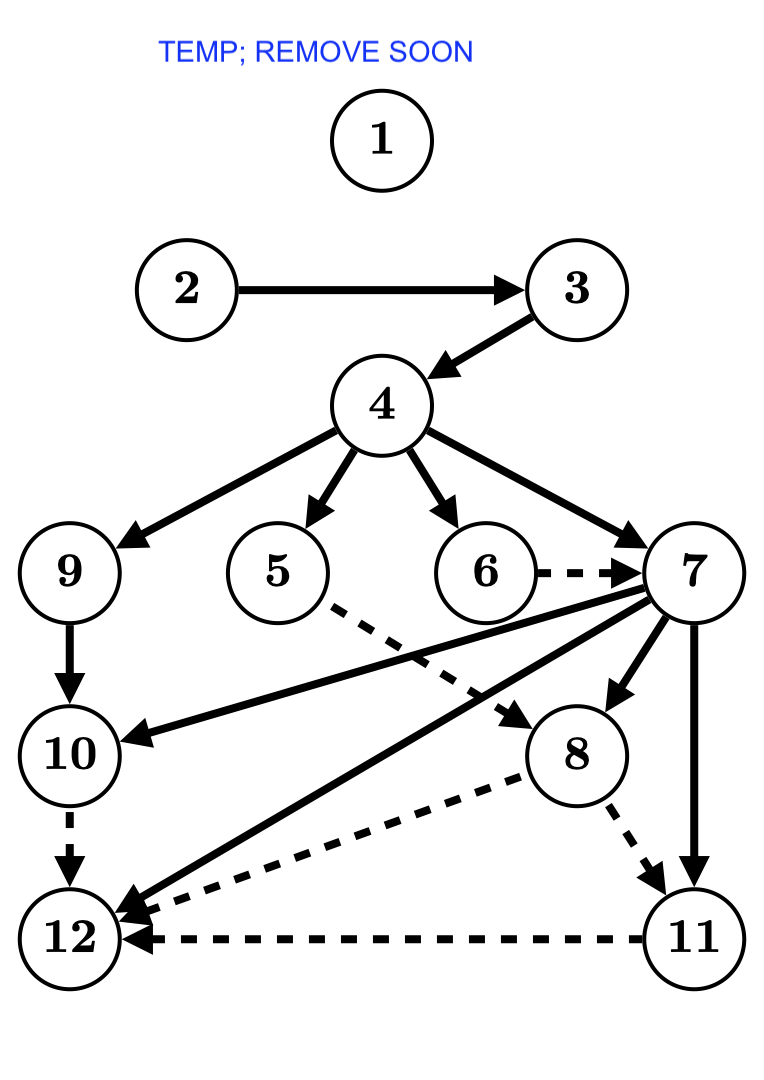
\includegraphics[width=\linewidth]{Interdependence.png}
    
    \newpage

    \textbf{Notes}:
    \interdependencenotes

    \mainmatter  % Now use arabic numerals for page numbers
}

%============= Index Pages ===============
\usepackage[
    totoc,
    columnsep=20pt,
    hangindent=8pt,
    subindent=20pt,
    subsubindent=30pt
]{idxlayout}

\makeindex[options= -s ../index-style.ist]

%======= Bibliography Formatting =========
% These two lines are here to ensure that URLs do not exceed the page by too much
\setcounter{biburllcpenalty}{7000}
\setcounter{biburlucpenalty}{8000}


%=========== Global Variables ============
\newcommand{\version}{0.13}
\newcommand{\volumenumber}{0}
\newcommand{\volumename}{Prerequisites}
\newcommand{\volumeimage}{cover/Venn Diagram.png}

%============= Formatting ================
\linespread{1.05}

%======== Theorem-Like Things ============
\renewcommand{\thetheoremhidden}{\arabic{part}.\arabic{chapter}.\arabic{section}.\arabic{theoremhidden}}
\renewcommand{\theexercisehidden}{\arabic{part}.\arabic{chapter}.\arabic{exercisehidden}}
\renewcommand{\theproblem}{\arabic{part}.\arabic{chapter}.\arabic{problem}}

%========= Front Matter Pages ============
% Quote page
\newcommand{\quotepagetext}{
    Aus dem Paradies, das Cantor uns geschaffen, soll uns niemand vertreiben k\"{o}nnen.\\
    (\textit{No one shall expel us from the Paradise that Cantor has created.})
}
\newcommand{\quotepageattribution}{David Hilbert, 1926}
\newcommand{\quotepagecitation}{\cite[p.~170]{hilbert_1926}}

% Preface
\newcommand{\prefacevolumetext}{
    To understand the subject material covered in the later volumes, the prerequisites and fundamentals must be understood. Volume 0 gives one sufficient knowledge to dive into the meat of abstract algebra. We cover basic set theory, functions/mappings, mathematical logic and proof writing, elementary number theory, and simple modular arithmetic, which should be plenty for one to understand the content covered in future volumes.
}
\newcommand{\prefacevolumedate}{22 March, 2023}

% Suggestions of use
\newcommand{\interdependencenotes}{
    \begin{itemize}
        \item All chapters of this volume are essential to understand for future volumes. Readers who are familiar with the content may skip this volume.
        \item Knowledge of chapter 1 is needed for both chapters 2 and 3.
        \item The only thing that is needed from chapter 2 for chapter 3 is knowledge of function notation. In particular, \myref{example-strong-induction-on-function} is the only example that requires knowledge of functions.
        \item Chapters 4, 5, and 6 are independent from the other chapters of this book.
        \item B\'{e}zout's Lemma (\myref{lemma-bezout}) is the sole result that is used from chapter 4 in chapter 5.
        \item Chapter 6 on polynomial algebra can be understood without reading any other chapters. B\'{e}zout's Lemma (\myref{lemma-bezout}) is casually mentioned in this chapter, but its knowledge is not assumed.
    \end{itemize}
}

%=========================================
\begin{document}
\frontmatterpages

%=========================================
\chapter{Set Theory}
Sets may be used to describe all of mathematics. All different kinds of mathematical structures may be described and explained using the notion of sets.

\section{Introduction to Sets}
\begin{definition}
    A \textbf{set}\index{set} is a collection of things. These things are called \textbf{elements}\index{element} of the set.
\end{definition}
If $x$ is an element of the set $S$, we write $x \in S$. This is read as ``$x$ is an element of the set $S$'' or ``$x$ is in $S$''. Otherwise, we write $x \notin S$. For convenience, if $x \in S$ and $y \in S$, we may write $x, y \in S$. If $z \in S$ also, we may write $x, y, z \in S$. The same applies for ``$\notin$''.

A set is often described by listing elements separated by commas, or by a characterizing property of its elements, within braces $\{ \ \}$. 
\begin{example}
    The collection $\{2, 3, 4, 5\}$ is a set which has 4 elements, namely 2, 3, 4, and 5.
\end{example}
Some sets may have infinitely many elements.
\begin{example}
    The integers $\{\dots, -3, -2, -1, 0, 1, 2, 3, \dots\}$ is a set with infinitely many elements. Here, the dots indicate that the pattern of integers goes on forever in both directions.
\end{example}

\begin{definition}
    A set with a finite number of elements is called a \textbf{finite set}\index{set!finite}. A set with an infinite number of elements is called an \textbf{infinite set}\index{set!infinte}.
\end{definition}

\begin{definition}\index{set!equality}
    Two sets $A$ and $B$ are equal if and only if they contain the same elements.
\end{definition}
\begin{example}
    The sets $A = \{1, 2, 3, 4\}$, $B = \{4, 3, 2, 1\}$, and $C = \{3, 4, 1, 2\}$ are equal to each other even though their elements are listed in a different order.
\end{example}
\begin{example}
    $\{1, 2, 3, 4\} \neq \{1, 2, 3, 5\}$ since the elements in the two sets differ.
\end{example}

What if a set has no elements?
\begin{definition}
    The \textbf{empty set}\index{set!empty} is the set $\{\}$ and is denoted by $\emptyset$. That is, $\emptyset = \{\}$.
\end{definition}

We introduce the idea of subsets.
\begin{definition}
    Let $A$ and $B$ be sets.
    \begin{itemize}
        \item $A$ is a \textbf{subset}\index{subset} of $B$ if and only if all elements of $A$ are elements of $B$. This is denoted by $A \subseteq B$.
        \item $A$ is a \textbf{proper subset}\index{subset!proper} if and only if $A$ is a subset of $B$ and $B$ contains at least one element not in $A$. In this case, we write $A \subset B$.
    \end{itemize}
\end{definition}
\begin{example}
    Let $A = \{1, 2\}$, $B = \{1, 2, 3\}$, $C = \{1, 4\}$, and $S = \{1, 2, 3\}$. Then $A \subseteq S$ since the elements of $A$, namely 1 and 2, also appear in $S$. Also $B \subseteq S$ since all elements of $B$ appear in $S$. However $C \not\subseteq S$ since 4 is not an element of $S$.

    We note that $B \not\subset S$ since $S$ does not contain an element that is not in $B$. But $A \subset S$ since 3 is not in $A$.
\end{example}

\begin{exercise}
    Let $S$ be a non-empty set. Determine whether the following statements are true or false.

    \begin{multicols}{2}
        \begin{enumerate}[label=(\alph*)]
            \item $\{1, 2\} \subset \{1, 2, 3, 4\}$
            \item $\{1, 2, 3\} \subseteq \{1, 2, 4\}$
            \item $\emptyset \subseteq \emptyset$
            \item $S \subset S$
            \item $S \in \{S, \emptyset\}$
            \item $\{S\} \notin \{S, \emptyset\}$
            \item $S \subseteq \{S, \emptyset\}$
            \item $\{S\} \subseteq \{S, \emptyset\}$
        \end{enumerate}
    \end{multicols}
\end{exercise}

There are some special sets that are so common that we have given special names and symbols.
\begin{itemize}
    \item $\mathbb{N}$ denotes the set of positive integers\index{set!of positive integers};
    \item $\mathbb{Z}$ denotes the set of integers\index{set!of integers} (from the German ``z\"{a}hlen", which means ``numbers");
    \item $\mathbb{Q}$ denotes the set of rational numbers\index{set!of rational numbers}; and
    \item $\mathbb{R}$ denotes the set of real numbers\index{set!of real numbers}.
\end{itemize}

\newpage

\section{Set Operations}
Certain operations could be performed on sets. We list the most commonly used ones here.

\begin{definition}
    The \textbf{union}\index{set!union} of two sets is the set of all objects that are a member of $A$, or $B$, or both. It is denoted $A \cup B$.
\end{definition}
\begin{example}
    $\{1, 2, 3\} \cup \{2, 3, 4\} = \{1, 2, 3, 4\}$.
\end{example}

\begin{definition}
    The \textbf{intersection}\index{set!intersection} of two sets is the set of all objects that are a member of \textit{both} the sets $A$ and $B$. It is denoted $A \cap B$.
\end{definition}
\begin{example}
    $\{1, 2, 3\} \cap \{2, 3, 4\} = \{2, 3\}$
\end{example}

\begin{definition}
    The \textbf{set difference}\index{set!difference} of $S$ and $A$, denoted $S \setminus A$, is the set of all members of $S$ that are not members of $A$.
\end{definition}
\begin{remark}
    Some authors will use the minus sign to denote the set difference, i.e. $A - B$ denotes the difference of $A$ and $B$ and is the same as $A \setminus B$ in this book.
\end{remark}
\begin{example}
    Let $A = \{1, 2, 3\}$ and $B = \{2, 3, 4\}$. Then $A \setminus B = \{1\}$ and $B \setminus A = \{4\}$.
\end{example}

\begin{definition}
    The \textbf{Cartesian Product}\index{Cartesian Product} of $A$ and $B$, denoted $A \times B$, is the set whose members are all possible ordered pairs $(a, b)$, where $a$ is an element of $A$ and $b$ is an element of $B$.
\end{definition}
\begin{example}
    Let $A = \{1, 2, 3\}$ and $B = \{4, 5\}$. Then
    \[
        A \times B = \{(1, 4), (1, 5), (2, 4), (2, 5), (3, 4), (3, 5)\}.
    \]
\end{example}
\begin{remark}
    In particular, if $A$ is a set, the Cartesian product $A \times A = A^2$, $A\times A \times A = A^3$, and so on.
\end{remark}

\begin{exercise}
    Let $S = \{1, 2, 3, 4\}$, $T = \{2, 3, 5\}$, $U = \{(2, 2), (3, 3), (5, 5)\}$. Determine whether the following statements are true or false.
    \begin{multicols}{2}
        \begin{enumerate}[label=(\alph*)]
            \item $S \cup T = \{1, 2, 3, 4, 5\}$
            \item $S \cup U = \{1, 2, 3, (5, 5)\}$
            \item $S \cap T = \{2, 3\}$
            \item $T \cap U = \emptyset$
            \item $S \setminus T = \{1, 4\}$
            \item $S \setminus \{1, 4\} = T$
            \item $T^2 = U$
            \item $U \subset (S \cup T)^2$
        \end{enumerate}
    \end{multicols}
\end{exercise}

\section{Set-Builder Notation}
Sometimes, some sets are too big or complex to list between the braces. In these cases, we use set-builder notation to describe the sets.
\begin{definition}
    A set $S$ with \textbf{set-builder notation}\index{set!builder notation} has the syntax
    \[
        S = \{\mathrm{expression} \ | \ \mathrm{rule}\},
    \]
    where the elements of $S$ are understood to be all values of the {\normalfont expression} that satisfy the {\normalfont rule}.
\end{definition}

\begin{example}
    Consider the infinite set of even integers, $E = \{\dots, -6, -4, -2, 0, 2, 4, 6, \dots\}$. It is often written as
    \[
        E = \{2n \vert n \in \mathbb{Z}\}.
    \]
    In this case, we may read the above expression as ``$E$ is the set of all things of form $2n$, where $n$ is an element of $\mathbb{Z}$''.

    There are equivalent forms of $E$:
    \[
        E = \{n \vert n \textrm{ is an even integer}\} = \{n \vert n = 2k, k \in \mathbb{Z}\}.
    \]

    Another common way of writing $E$ is
    \[
        E = \{n \in \mathbb{Z} \vert n \textrm{ is even}\}
    \]
    where it could be read as ``$E$ is the set of all $n$ in $\mathbb{Z}$ such that $n$ is even''.
\end{example}
\begin{remark}
    Some authors use the colon instead of the bar, i.e. $S = \{\mathrm{expression} \ : \ \mathrm{rule}\}$. We use the bar.
\end{remark}

\begin{example}
    The set $S = \{x \in \mathbb{R} \ | \ x \geq 0 \}$ is the set of all non-negative real numbers.
\end{example}

\section{Cardinality}
\begin{definition}
    The \textbf{cardinality}\index{cardinality} of a set $S$, denoted by $|S|$, is a measure of the number of elements of the set.
    \begin{itemize}
        \item If $S$ is finite, then $|S|$ is the number of elements in $S$.
        \item If $S$ is infinite, then we write $|S| = \infty$.
    \end{itemize}
\end{definition}
\begin{remark}
    Of course, the notion that $|S| = \infty$ is poorly defined in other contexts. However, for this book, this definition would be sufficient for most of the things we wish to accomplish.
\end{remark}
\begin{example}
    The set $A = \{1, 2, 3\}$ has cardinality 3, i.e. $|A| = 3$.
\end{example}
\begin{example}
    The empty set $\emptyset$ has cardinality 0 since it has no elements, i.e. $|\emptyset| = 0$.
\end{example}
\begin{example}
    The set of integers has infinite elements, so we write $|\mathbb{Z}| = \infty$ for this book.
\end{example}

\begin{exercise}
    Let the sets
    \begin{align*}
        S &= \{x \in \mathbb{Q} \vert x \leq 0\}\\
        T &= \{y \in \mathbb{Z} \vert -2 \leq y \leq 10 \text{ and } y \text{ is an even number} \}
    \end{align*}
    List the elements in the set $S \cap T$.
\end{exercise}

%=========================================
\chapter{Functions / Maps}
Functions (or maps) play a fundamental role in mathematics. Functions compare and relate different kinds of mathematical structures to each other, and provide a way to relate elements from one structure to another.

\section{Introduction to Functions / Maps}
\begin{definition}
    A \textbf{function}\index{function} (or a \textbf{map}\index{map}) $f$ from a set $X$ to a set $Y$ assigns each value in $X$ to exactly one element in $Y$, and is denoted by $f: X \to Y$.
\end{definition}
\begin{definition}
    For a function $f: X \to Y$, the set $X$ is called the \textbf{domain}\index{domain} of the function and the set $Y$ is called the \textbf{codomain}\index{codomain} of the function.
\end{definition}
\begin{example}
    Consider the simple function $f: \mathbb{Z} \to \mathbb{Q}$ where $f(n) = \frac1n$. In this case, $f$ has a domain of $\mathbb{Z}$, i.e. the integers, and a codomain of $\mathbb{Q}$, i.e. the rational numbers.

    We may evaluate the function $f$ at $2 \in \mathbb{Z}$ to get the resulting value of $f(2) = \frac12$.
\end{example}

\textbf{Arrow notation}\index{function!arrow notation} can also be used to define the rule of a function. There is no good way of defining how to use arrow notation, but some examples should help illustrate the basic idea.
\begin{example}
    Consider $f: \mathbb{N} \to \mathbb{Q}$ where $f(n) = \frac1n$. We may write this more succinctly as $f: \mathbb{N} \to \mathbb{Q}, n \mapsto \frac1n$. Specifically, $n \mapsto \frac1n$ is read as ``$n$ maps to $\frac1n$''.
    
    It is important to note that $\to$ is used to indicate the domain and codomain, and that $\mapsto$ indicates how an element in the domain is `transformed' into an element in the codomain.
\end{example}
\begin{example}
    The function $g: \mathbb{R} \to \mathbb{R}$ where $g(x) = x^2 - 2x + 1$ can be more succinctly written as $g: \mathbb{R} \to \mathbb{R}, x \mapsto x^2 - 2x + 1$.
\end{example}
\begin{example}
    Let $h: \mathbb{Z} \to \mathbb{R}$ where $h(x^2) = x$. This can be written succinctly as either $h: \mathbb{Z} \to \mathbb{R}, x^2 \mapsto x$ or $h: \mathbb{Z} \to \mathbb{R}, n \mapsto \sqrt n$.
\end{example}

We now look at the definition of the image and range.
\begin{definition}
    Let $f: X \to Y$ be a function, and $x \in X$.
    \begin{itemize}
        \item The \textbf{image}\index{function!image} of an element $x \in X$ under the function $f$ is denoted $f(x)$ and is defined to be the value after applying $f$ to $x$.
        \item The \textbf{image} or \textbf{range}\index{function!range} of $f$ is denoted by either $\im f$ or $f(X)$ and is the set of the images of all elements in the domain.
    \end{itemize}
\end{definition}
\begin{example}
    Consider the function $f: \mathbb{Z} \to \mathbb{Z}, n \mapsto 1$.
    \begin{itemize}
        \item The image of 0 under $f$ is 1.
        \item The range/image of $f$ is the \textit{set} $\{1\}$, i.e. $\im f = f(\mathbb{Z}) = \{1\}$.
    \end{itemize}
    It is important to note that the image of an element is a single element, while the image of the function is a set.
\end{example}
\begin{example}
    Consider the function $g: \mathbb{Z} \to \mathbb{Z}, n \mapsto |n|$, where $|n|$ denotes the absolute value of $n$.
    \begin{itemize}
        \item The image of 2 under $g$ is $|2| = 2$.
        \item The image of -3 under $g$ is $|-3| = 3$.
        \item The image of 0 under $g$ is $|0| = 0$.
    \end{itemize}
    The range of the function $g$ is the set of non-negative integers, i.e. $\im g = g(\mathbb{Z}) = \mathbb{N} \cup \{0\}$.
\end{example}

\begin{exercise}
    Let a function $f: \{1, 2, 3\} \to \{1, 4, 9, 16, 25\}$ be given by the relation $f(x) = x^2$.
    \begin{enumerate}[label=(\roman*)]
        \item Use arrow notation to write a definition for $f$.
        \item State the domain, codomain, and range of $f$.
        \item What is the image of 2 under $f$?
        \item Is the function $g: \{1, 2, 3\} \to \{1, 8\}, x \mapsto x^3$ \textit{valid}?
    \end{enumerate}
\end{exercise}

We end this section with defining equality of two functions.
\begin{definition}
    Let $f: A \to B$ and $g: C \to D$ be functions. Then $f$ and $g$ are \textbf{equal}\index{function!equality} if and only if
    \begin{itemize}
        \item $A = C$ and $B = D$; and
        \item for all $x \in A = C$, we have $f(x) = g(x)$.
    \end{itemize}
    We denote $f = g$ if the two functions are equal.
\end{definition}
In other words, two functions $f$ and $g$ are equal if their domain and codomain sets are the same and their output values agree on the whole domain.
\begin{example}
    Consider the functions $f: \mathbb{Z} \to \mathbb{Z}, x \mapsto (x-1)^2$ and $g: \mathbb{Z} \to \mathbb{Z}, x \mapsto x^2 - 2x + 1$. Since the two functions' domains and codomains are the same, and because $(x-1)^2 = x^2 - 2x + 1$, thus $f = g$.
\end{example}
\begin{example}
    The functions $f: \mathbb{Z} \to \mathbb{R}, x \mapsto (x-1)^2$ and $g: \mathbb{Z} \to \mathbb{Q}, x \mapsto x^2 - 2x + 1$ are not equal because their codomains differ.
\end{example}

\section{Well-Defined Functions}
\begin{definition}
    A function $f: X \to Y$ is \textbf{well-defined} if and only if for each $x \in X$ there is a unique $y \in Y$ such that $f(x) = y$.
\end{definition}
Informally, \textit{similar inputs} produce \textit{identical outputs} for a well-defined function.
\begin{remark}
    Functions that are not well-defined are called `ambiguous' or `ill-defined' functions.
\end{remark}
\begin{remark}
    If a function is not well-defined, then it is not a valid function.
\end{remark}

\begin{example}
    Let $S_1$ and $S_2$ be sets, and let $S = S_1 \cup S_2$. Let $f: S \to \{1, 2\}$, such that
    \[
        f(x) = \begin{cases}
            1 & \textrm{ if } x \in S_1\\
            2 & \textrm{ if } x \in S_2
        \end{cases}
    \]
    Then $f$ is well-defined if $S_1 \cap S_2 = \emptyset$. For example, if $S_1 = \{1, 2\}$ and $S_2 = \{3, 4\}$, then $f$ is well-defined.
    
    On the other hand, if $S_1 \cap S_2 \neq \emptyset$, then $f$ is not well-defined. For example, if $S_1 = \{1, 2\}$ and $S_2 = \{2, 3\}$, then $f(2) = 1$ and $f(2) = 2$ simultaneously.
\end{example}

\begin{exercise}
    Is the function
    \[
        f: \mathbb{Q} \to \mathbb{Z},\;\frac pq \mapsto p + q    
    \]
    well-defined?
\end{exercise}

\section{Function Composition}
\begin{definition}
    Let $f: X \to Y$ and $g: Y \to Z$ be functions. Then \textbf{composing $f$ with $g$}\index{function!composition} produces a function $h: X \to Z$ where $h(x) = f(g(x))$. We denote $h = f \circ g$ where $\circ$ is the function composition operator.
\end{definition}
\begin{remark}
    We may also alternatively write $fg$ in place of $f \circ g$.
\end{remark}

It is important to note the following about function composition.
\begin{itemize}
    \item Function composition is associative\index{function!composition!associative}. That is, if $f$, $g$, and $h$ are composable, then $f \circ (g \circ h) = (f \circ g) \circ h$. As parentheses do not change the result, they are usually omitted.
    \item The composition $f \circ g$ is only meaningful if the codomain of $g$ is a subset of the domain of $f$. That is, if $f: A \to B$ and $g: C \to D$, then $f \circ g$ is only meaningful if $\im g \subseteq A$.
\end{itemize}

\begin{exercise}
    Let $f: \mathbb{R} \to \mathbb{R}$ and $g: \mathbb{R} \to \mathbb{R}$. Write down the rule of the function $fg$ if $f(x) = x^2 - x + 1$ and $g(y) = \frac1{y^2+1}$.
\end{exercise}

\section{Injective, Surjective, and Bijective Functions}
\begin{definition}
    A function $f: X \to Y$ is \textbf{injective}\index{function!injective} (or \textbf{one-to-one}\index{function!one-to-one}) if $f(x_1) = f(x_2)$ implies $x_1 = x_2$.
\end{definition}
\begin{remark}
    Equivalently, if $x_1 \neq x_2$ then $f(x_1) \neq f(x_2)$ for all $x_1$ and $x_2$ in $X$.
\end{remark}
\begin{example}
    Consider $f: \mathbb{N} \to \mathbb{N}, n \mapsto n^2$. We show that $f$ is injective.
    
    Note that if $n_1, n_2 \in \mathbb{N}$ are such that $f(n_1) = n_1^2 = f(n_2) = n_2^2$ then $n_1 = n_2$ (since $n_1, n_2 > 0$ so taking the square root is okay). Thus $f$ is injective.
\end{example}
\begin{example}
    Consider instead $g: \mathbb{Z} \to \mathbb{Z}, n \mapsto n^2$. Then $g$ is not injective since $g(-2) = g(2) = 4$.
\end{example}

\begin{definition}
    A function $f: X \to Y$ is \textbf{surjective}\index{function!surjective} (or \textbf{onto}\index{function!onto}) if for every $y \in Y$, there exists an $x \in X$ (called the \textbf{pre-image}\index{function!pre-image} of $y$) such that $f(x) = y$.
\end{definition}
\begin{remark}
    Equivalently, the image of $f$ is equal to its codomain, i.e. $\im f = Y$.
\end{remark}
\begin{example}
    Let $S$ denote the set of non-negative real numbers, i.e. $S = \{x\in\mathbb{R} | x \geq 0\}$. Consider the function $f: \mathbb{R} \to S, x \mapsto x^2$. We show that $f$ is surjective.

    Let $y \in S$. Note that $\sqrt{y} \in \mathbb{R}$ since $y$ is a non-negative real number. Observe that $f(\sqrt{y}) = (\sqrt y)^2 = y$. Thus any $y \in Y$ has a pre-image $\sqrt y \in X$. Thus $f$ is surjective.
\end{example}
\begin{example}
    Consider instead the function $g: \mathbb{R} \to \mathbb{R}, x \mapsto x^2$. Then $g$ is not surjective because there is no real number $x \in \mathbb{R}$ such that $g(x) = -1$.
\end{example}

\begin{definition}
    A function is \textbf{bijective}\index{function!bijective} (or a \textbf{bijection}\index{bijection} or a \textbf{one-to-one correspondence}\index{function!one-to-one!correspondence}) if the function is both injective and surjective.
\end{definition}
\begin{example}
    Consider the function $f: \mathbb{R} \to \mathbb{R}, x \mapsto x^3$. We show that $f$ is bijective.
    \begin{itemize}
        \item \textbf{Injective}: Let $a, b \in \mathbb{R}$ such that $f(a) = f(b)$, i.e. $a^3 = b^3$. Clearly we may take the cube root on both sides to yield $a = b$, so $f$ is injective.
        \item \textbf{Surjective}: Let $y \in \mathbb{R}$. Set $x=y^{\frac13}$. Note $x \in \mathbb{R}$ and observe that $f(x) = \left(y^{\frac13}\right)^3 = y$. Thus $y$ has a pre-image of $y^{\frac13}$ in $\mathbb{R}$ and so $f$ is surjective.
    \end{itemize}
    Since $f$ is both injective and surjective it is thus bijective.
\end{example}

\begin{definition}
    Let $A$ and $B$ be sets. Then $A$ and $B$ are \textbf{equinumerous}\index{set!equinumerous} if there exists a bijective function $f: A \to B$. In this case, $A$ and $B$ have the same cardinality, i.e., $|A| = |B|$.
\end{definition}
\begin{remark}
    It should be noted that bijectivity is also implied if the function $f: X \to Y$ is injective and the sets $X$ and $Y$ are equinumerous.
\end{remark}

\begin{exercise}
    Define the function $f: \mathbb{N} \to \mathbb{Z}$ such that
    \[
        f(x) = \begin{cases}
            \frac{x}{2} & \text{ if } x \text{ is even}\\
            \frac{1-x}{2} & \text{ if } x \text{ is odd} 
        \end{cases}
    \]
    By considering $f$, prove that $|\mathbb{N}| = |\mathbb{Z}|$.
\end{exercise}

%=========================================
\chapter{Mathematical Logic and Proof Writing}
The heart of mathematics is in its logical statements. These statements are used to produce a series of logical steps to prove a claim. We explore the basics of logic and proof writing here.

\section{Mathematical Statements}
\begin{definition}
    A \textbf{(mathematical) statement}\index{statement} (or \textbf{proposition}\index{proposition}) is a sentence that is definitely true or definitely false, but not both.
\end{definition}
\begin{remark}
    A statement can be written in English, or using mathematical notation.
\end{remark}
\begin{example}
    The sentence ``every square with length $x$ has area $x^2$'' is a true mathematical statement.
\end{example}
\begin{example}
    The sentence ``every circle with radius $x$ has area $x^2$'' is a false mathematical statement.
\end{example}
\begin{example}
    The sentence ``$12 \in \mathbb{Z}$'' is a true mathematical statement.
\end{example}
\begin{example}
    The sentence ``$\sqrt2 \in \mathbb{Z}$'' is a false mathematical statement.
\end{example}

We may name statements using variables like $P$, $Q$, $R$, etc.
\begin{example}
    If
    \begin{align*}
        P: &\ \text{Every odd number is one more than an even number}\\
        Q: &\ \text{Every triangle has sides of equal length}\\
        R: &\ \frac12 \in \mathbb{Q}
    \end{align*}
    then $P$ is true, $Q$ is false, and $R$ is true.
\end{example}

There are a few operations\index{logical operation} that may be carried out on mathematical statements. For the following, assume $P$ and $Q$ are mathematical statements.
\begin{itemize}
    \item \textbf{Logical NOT}\index{logical operation!NOT}: Uses the symbol $\lnot$. The statement $\lnot P$ is read as ``not $P$''.
    \item \textbf{Logical AND}\index{logical operation!AND}: Uses the symbol $\land$. The statement $P\land Q$ is read as ``$P$ and $Q$''.
    \item \textbf{Logical OR}\index{logical operation!OR}: Uses the symbol $\lor$. The statement $P\lor Q$ is read as ``$P$ or $Q$''.
    \item \textbf{Conditional}\index{logical operation!conditional}: Uses the symbol $\implies$. The statement $P \implies Q$ is read as ``$P$ implies $Q$''.  
\end{itemize}
\begin{example}
    If $P$ is the statement ``3 is an odd number'' and $Q$ is the statement ``4 is an odd number'', then
    \begin{itemize}
        \item $P\land Q$ is ``3 is an odd number \textbf{and} 4 is an odd number'', which is false;
        \item $P\lor Q$ is ``3 is an odd number \textbf{or} 4 is an odd number'', which is true; and
        \item $\lnot Q$ is ``4 is \textbf{not} an odd number'', which is true.
    \end{itemize}
\end{example}
\begin{exercise}
    Let $P$ be ``1 is a positive number'', $Q$ be ``$-1 > 0$'', and $R$ be ``1 is an odd number''. Is the statement ``$\lnot((P\lor Q)\land R)$ is false'' true?
\end{exercise}

We use \textbf{truth tables}\index{truth table} to explore the relationships between statements and operators. They list all possibilities of the truth or falsity of the statements $P$ and $Q$, and then write the truth for each of the combinations with operations. In a truth table, we denote true statements by ``T'' and false statements by ``F''. For example, the truth table for the logical AND operator is:
\begin{table}[h]
    \centering
    \begin{tabular}{|l|l||l|}
        \hline
        $P$ & $Q$ & $P\land Q$ \\ \hline
        F   & F   & F          \\ \hline
        F   & T   & F          \\ \hline
        T   & F   & F          \\ \hline
        T   & T   & T          \\ \hline
    \end{tabular}
\end{table}

The truth table for the logical OR operator is:
\begin{table}[h]
    \centering
    \begin{tabular}{|l|l||l|}
        \hline
        $P$ & $Q$ & $P\lor Q$ \\ \hline
        F   & F   & F         \\ \hline
        F   & T   & T         \\ \hline
        T   & F   & T         \\ \hline
        T   & T   & T         \\ \hline
    \end{tabular}
\end{table}

The truth table for the logical NOT operator is:
\begin{table}[h]
    \centering
    \begin{tabular}{|l||l|}
        \hline
        $P$ & $\lnot P$ \\ \hline
        F   & T         \\ \hline
        T   & F         \\ \hline
    \end{tabular}
\end{table}

We motivate the truth table for the conditional by considering the statements ``you pass the exam'' and ``you pass the course'', which we will denote by $P$ and $Q$ respectively. So $P \implies Q$ would be ``if you pass the exam then you pass the course''.
\begin{itemize}
    \item If $P$ and $Q$ are true, then that means that you passed the exam and passed the course. Hence, ``if you pass the exam then you pass the course'' is \textbf{true}, meaning $P \implies Q$ is true.
    \item If $P$ is true and $Q$ is false, then that means that you passed the exam but failed the course. Hence, the promise that ``if you pass the exam then you pass the course'' is broken, meaning $P \implies Q$ is false.
    \item Now consider the third case when $P$ is false but $Q$ is true. This means that you failed the exam but passed the course. This does not mean that the promise was broken; you could have passed the course through other means. The only promise was that if you pass the exam then you pass the course; the promise was not that passing the exam was the \textit{only} way of passing the course. Since the promise was not broken, thus the promise was kept, so $P \implies Q$ is true.
    \item Finally we consider the case when $P$ and $Q$ are both false: you failed the exam and failed the course. The promise certainly was not broken in this case, so $P \implies Q$ is true.
\end{itemize}
\begin{remark}
    A conditional statement that is true by the virtue of the fact that $P$ is false is called \textbf{vacuously true}\index{vacuously true}.
\end{remark}

\newpage

In summary, the truth table for the conditional is:
\begin{table}[h]
    \centering
    \begin{tabular}{|l|l||l|}
        \hline
        $P$ & $Q$ & $P\implies Q$ \\ \hline
        F   & F   & T             \\ \hline
        F   & T   & T             \\ \hline
        T   & F   & F             \\ \hline
        T   & T   & T             \\ \hline
    \end{tabular}
\end{table}

\begin{exercise}
    Let $P$ and $Q$ be statements. Draw the truth table for $P \land (\lnot Q)$.
\end{exercise}

We end this section by introducing the idea of the \textbf{biconditional}\index{logical operation!biconditional}.
\begin{definition}
    Let $P$ and $Q$ be mathematical statements. If both $(P \implies Q)$ and $(Q \implies P)$ are true, then we write $(P \iff Q)$. In other words, $(P \iff Q) \equiv ((P \implies Q) \land (Q \implies P))$.
\end{definition}
\begin{remark}
    The statement $(P \iff Q)$ can be written in several ways in English:
    \begin{itemize}
        \item $P$ if and only if $Q$;
        \item $P$ is a necessary and sufficient condition for $Q$; or
        \item $P$ is equivalent to $Q$.
    \end{itemize}
\end{remark}

\newpage

The truth table for the biconditional is:
\begin{table}[h]
    \centering
    \begin{tabular}{|l|l||l|}
        \hline
        $P$ & $Q$ & $P\iff Q$ \\ \hline
        F   & F   & T         \\ \hline
        F   & T   & F         \\ \hline
        T   & F   & F         \\ \hline
        T   & T   & T         \\ \hline
    \end{tabular}
\end{table}

\begin{exercise}
    Suppose $n$ is an integer. Let $P$ be the statement ``$n$ is a multiple of 5'' and $Q$ be the statement ``the last digit of $n$ is 0 or 5''. Let the statement $R = (P \iff Q)$.
    \begin{enumerate}[label=(\roman*)]
        \item Write the statement $R$ in English.
        \item Is the statement $R$ true? Justify your answer.
    \end{enumerate}
\end{exercise}

\section{Properties of Logical Operators}
A central idea of this section is that every mathematical statement can be built from just $\land$, $\lor$, and $\lnot$.

\begin{example}
    We show that $(P \implies Q) \equiv (\lnot P) \lor Q$ by considering the truth table $(\lnot P) \lor Q$.
    \begin{table}[h]
        \centering
        \begin{tabular}{|l|l||l||l|}
            \hline
            $P$ & $Q$ & $\lnot P$ & $(\lnot P) \lor Q$ \\ \hline
            F   & F   & T         & T                  \\ \hline
            F   & T   & T         & T                  \\ \hline
            T   & F   & F         & F                  \\ \hline
            T   & T   & F         & T                  \\ \hline
        \end{tabular}
    \end{table}

    \newpage
    
    By inspection, we see that $(\lnot P) \lor Q$ has the same truth table as $P \implies Q$. Thus $(P \implies Q) \equiv (\lnot P) \lor Q$.
\end{example}
\begin{remark}
    We separate the intermediate value(s) (e.g. $\lnot P$ in the above example) from the rest by drawing a double line to the sides of the intermediate values.
\end{remark}

\begin{example}
    We show that $(P \iff Q) \equiv (P \land Q) \lor ((\lnot P) \land (\lnot Q))$. For brevity, let $R = (\lnot P) \land (\lnot Q)$.
    \begin{table}[h]
        \centering
        \begin{tabular}{|l|l||l|l|l|l||l|}
            \hline
            $P$ & $Q$ & $\lnot P$ & $\lnot Q$ & $P \land Q$ & $R$ & $(P \land Q) \lor R$ \\ \hline
            F   & F   & T         & T         & F           & T   & T                    \\ \hline
            F   & T   & T         & F         & F           & F   & F                    \\ \hline
            T   & F   & F         & T         & F           & F   & F                    \\ \hline
            T   & T   & F         & F         & T           & F   & T                    \\ \hline
        \end{tabular}
    \end{table}

    By inspection of the truth table we establish the required result.
\end{example}

\begin{exercise}
    Show that
    \[
        ((\lnot P) \iff Q) \equiv (P \implies (\lnot Q)) \land ((\lnot Q) \implies P)
    \]
    by drawing a truth table.
\end{exercise}

We note some important properties of logical operators.
\begin{itemize}
    \item \textbf{Contrapositive}\index{contrapositive}: $(P \implies Q) \equiv ((\lnot Q) \implies (\lnot P))$
    \item \textbf{De Morgan's Laws}: \begin{itemize}
        \item $(\lnot (P \land Q)) \equiv ((\lnot P) \lor (\lnot Q))$
        \item $(\lnot (P \lor Q)) \equiv ((\lnot P) \land (\lnot Q))$
    \end{itemize}

    \newpage

    \item \textbf{Commutativity of AND and OR}: \begin{itemize}
        \item $P \land Q \equiv Q \land P$
        \item $P \lor Q \equiv Q \lor P$
    \end{itemize}
    \item \textbf{Associativity of AND and OR}: \begin{itemize}
        \item $P \land (Q \land R) \equiv (P \land Q) \land R$
        \item $P \lor (Q \lor R) \equiv (P \lor Q) \lor R$
    \end{itemize}
    \item \textbf{Distributive Rules}: \begin{itemize}
        \item $P \land (Q \lor R) \equiv (P \land Q) \lor (P \land R)$
        \item $P \lor (Q \land R) \equiv (P \lor Q) \land (P \lor R)$
    \end{itemize}
\end{itemize}
\begin{remark}
    The most important one of these properties would arguably be the contrapositive. We will use this result several times later and in later volumes.
\end{remark}
\begin{exercise}
    Simplify the statement
    \[
        ((P \lor \lnot Q) \land \lnot R) \lor ((P \lor \lnot Q) \land (P \lor R) \land (P \lor \lnot R))
    \]
    into a statement that uses only \textbf{three} operators in total.
\end{exercise}

\section{Quantifiers}
\begin{definition}
    The \textbf{universal quantifier}\index{quantifier!universal} is $\forall$ and is read as ``for all''.
\end{definition}
\begin{example}
    The statement ``for every integer $n$, the integer $2n$ is an even number'' can be written as ``$\forall n \in \mathbb{Z}, 2n$ is even''.
\end{example}

\begin{definition}
    The \textbf{existential quantifier}\index{quantifier!existential} is $\exists$ and is  read as ``there exists''.
\end{definition}
\begin{example}
    The statement ``there exists a subset of $\mathbb{Z}$ which has 10 elements'' is equivalent to ``$\exists S \subseteq \mathbb{Z} \text{ such that } |S| = 10$''.
\end{example}
\begin{remark}
    We usually shorten the ``such that'' as ``s.t.'', so the above statement is written symbolically as ``$\exists S \subseteq \mathbb{Z} \text{ s.t. } |S| = 10$''.
\end{remark}

We can also combine the quantifiers together with logical operators.
\begin{example}
    The statement ``every odd integer is one less than an even integer'' can be written as ``$\forall n \in \mathbb{Z}$, $\exists k \in \mathbb{Z} \text { s.t. } n = 2k - 1$''.
\end{example}
\begin{example}
    Fermat's Last Theorem, which states that for all integers $n\geq 3$ the equation $x^n + y^n = z^n$ has no solution for $x, y, z \in \mathbb{N}$, can be written as
    \[
        \left[(n \in \mathbb{Z}) \land (n \geq 3)\right] \implies \left[\forall x, y, z \in \mathbb{N}, x^n + y^n \neq z^n\right].
    \]
    It should be noted that when translating from English to \textit{symbolic writing}, we may need to change some things around.
\end{example}

\begin{exercise}
    Convert the statement
    \begin{quote}
        for all positive integers $n > 2$ there exist integers $a$ and $b$ such that $a^3 + b^4 = n^5$
    \end{quote}
    into symbolic notation using quantifiers and logical operators.
\end{exercise}

\newpage

We now look at negating quantifiers\index{quantifier!negation}. Note that
\begin{itemize}
    \item $\lnot(\forall x, P(x)) \equiv \exists x \text{ s.t. } \lnot P(x)$; and
    \item $\lnot(\exists x \text{ s.t. } P(x)) \equiv \forall x, \lnot P(x)$.
\end{itemize}
\begin{example}
    Consider the statement ``for every integer $n$, the integer $2n$ is even''. One may write that using quantifiers as
    \[
        \forall n \in\mathbb{Z}, 2n \text{ is even}.
    \]
    Negating the above statement would make it
    \[
        \exists n \in \mathbb{Z}, 2n \text{ is not even},
    \]
    i.e., ``there exists an integer $n$ such that $2n$ is odd''.
\end{example}

We also note that $\lnot(P \implies Q) \equiv P \land \lnot Q$. We leave verifying this identity as an exercise to the reader.

\begin{example}
    Consider the statement ``if $n$ is odd then $n^3$ is odd''. We may write this using logical operators as ``($n$ is odd) $\implies$ ($n^3$ is odd)''. The negation of such a statement would hence be ``$n$ is odd \textbf{and} $n^3$ is \textbf{not} odd'', i.e. ``$n$ is odd and $n^3$ is even''.
\end{example}

\begin{exercise}
    Consider the statement ``if $x$ is a non-zero real number, then there exists a real number $y$ such that $xy = 1$''.
    \begin{enumerate}[label=(\roman*)]
        \item Write down two statements $P$ and $Q$ in symbols such that the above statement is $P \implies Q$.
        \item Negate the above statement, writing your answer in symbolic notation.
    \end{enumerate}
\end{exercise}

\newpage

\section{Hierarchy of Mathematical Results}
Mathematical statements often have a certain `tier' attached to them. We look at the hierarchy of some of these `tiers'.
\begin{itemize}
    \item \textbf{Proposition}\index{proposition}: A proposition can be thought of as a general proven result. Equivalent names for a proposition are ``\textbf{Claim}'' or ``\textbf{Observation}''.
    \item \textbf{Lemma}\index{lemma}: A lemma can be thought of as a `small' proven result that can help build other mathematical results. For example, Euclid's lemma that ``if a prime $p$ divides the product $ab$ of two integers $a$ and $b$, then $p$ must divide at least one of those integers $a$ or $b$'' is used in the proof of the Fundamental Theorem of Arithmetic.
    \item \textbf{Theorem}\index{theorem}: A theorem can be thought of as a `big' proven result. For example, the Fundamental Theorem of Arithmetic is core to arithmetic as it describes how integers can be uniquely decomposed into its prime factors.
    \item \textbf{Corollary}\index{corollary}: A corollary is said to be a `follow-up result' from a theorem. These results usually follow `very quickly' from a theorem or a proposition. For example, the AM-GM inequality is a corollary of the Pythagorean theorem.
    \item \textbf{Conjecture}\index{conjecture}: A conjecture is a mathematical statement whose truth or falsity is not known.
\end{itemize}

\section{Mathematical Proof Techniques}
\subsection{Direct Proof}
In essence, a direct proof\index{proof!direct} for the statement ``if $P$ then $Q$'' would involve
\begin{enumerate}
    \item supposing $P$ is true, (usually written as ``suppose $P$'')
    \item unpacking $P$ via definitions; making appropriate calculations and logical arguments; repacking $Q$ via definitions,
    \item concluding that $Q$ is true. (usually written as ``thus $Q$'')
\end{enumerate}
\begin{example}
    We look at a proof of the statement ``if the integer $n$ is odd then $n^2$ is odd''.
    \begin{proof}
        Suppose $n\in\mathbb{Z}$ is an odd number.
        
        Then $n$ can be written in the form $n = 2k + 1$ where $k$ is an integer. Hence $n^2 = (2k+1)^2 = 4k^2 + 4k + 1$. Note $4k^2 + 4k + 1 = 2(2k^2 + 2k) + 1$, so $n^2$ is one more than a multiple of 2.
        
        Thus $n^2 = 2(2k^2 + 2k) + 1$ is odd.
    \end{proof}
\end{example}

\begin{example}
    We look at a proof of the statement ``if $n$ is an integer then $1 + (-1)^n(2n-1)$ is a multiple of 4''.
    \begin{proof}
        Suppose $n$ is an integer. Then, $n$ is either odd or even. We look at two cases.
        \begin{itemize}
            \item When $n$ is odd, $(-1)^n = -1$ and $n = 2k+1$ for some integer $k$. Thus
            \[
                1 + (-1)^n(2n-1) = 1 - (2(2k+1)-1) = -4k
            \]
            which is a multiple of 4.
            \item When $n$ is even, $(-1)^n = 1$ and $n = 2k$ for some integer $k$. Thus
            \[
                1 + (-1)^n(2n-1) = 1 + (2(2k)-1) = 4k
            \]
            which is a multiple of 4.
        \end{itemize}
        Hence, in both cases, $1 + (-1)^n(2n-1)$ is a multiple of 4.
    \end{proof}
\end{example}

\begin{exercise}
    Prove that $m + n$ is even if the integers $m$ and $n$ have the same parity (i.e., both odd or both even). 
\end{exercise}

\subsection{Contrapositive Proof}
We now look at a \textbf{contrapositive proof}\index{proof!contrapositive}. Recall that $(P \implies Q) = (\lnot Q \implies \lnot P)$. Hence, a contrapositive proof for the statement ``if $P$ then $Q$'' would involve
\begin{enumerate}
    \item supposing $\lnot Q$ is true,
    \item working towards showing that $\lnot P$ is true,
    \item concluding that $\lnot P$ is true.
\end{enumerate}

Generally, we would want to prove in the direction from simplicity to complexity. So if $P$ is more complex than $Q$, we may consider using a contrapositive proof.

\begin{example}\label{example-if-(n-1)(n-5)-is-even-then-n-is-odd}
    Suppose $n$ is an integer. We prove the statement ``if $n^2 - 6n + 5$ is even, then $n$ is odd''. We note that a direct proof would be tedious and problematic. Using a contrapositive proof would be easier.
    
    We first note that the contrapositive statement that we want to prove is ``if $n$ is \textbf{not} odd, then $n^2 - 6n + 5$ is \textbf{not} even'', that is, ``if $n$ is even, then $n^2 - 6n + 5$ is odd''.
    \begin{proof}
        We consider a proof by contrapositive.
        
        Suppose $n$ is even. Then $n = 2k$ where $k$ is an integer. Note
        \begin{align*}
            n^2 - 6n + 5 &= (2k)^2 - 6(2k) + 5\\
            &= 4k^2 - 12k + 5\\
            &= (4k^2 - 12k + 4) + 1\\
            &= 2(2k^2 - 6k + 2) + 1
        \end{align*}
        which means that $n^2 - 6n + 5$ is one more than a multiple of 2, which hence means $n^2 - 6n + 5$ is odd.
    \end{proof}    
\end{example}

\begin{example}
    Suppose $x$ and $y$ are real numbers. We prove the statement ``$x \leq y$ if $x^3 + xy^2 \leq x^2y + y^3$'' using a contrapositive proof.
    
    We first note that the contrapositive statement that we want to prove is ``if $x > y$ then $x^3 + xy^2 > x^2y + y^3$''.

    \begin{proof}
        We consider a proof by contrapositive.
        
        Assume $x > y$. Then $x - y > 0$. Also, since $x > y$, thus $x$ and $y$ are not both zero. Hence $x^2 + y^2 > 0$.
        Observe
        \[
            (x-y)(x^2+y^2) > 0 \times (x^2+y^2) = 0        
        \]
        so $(x-y)(x^2+y^2) = x^3 + xy^2 - x^2y - y^3 > 0$. Therefore $x^3 + xy^2 > x^2y + y^3$.
    \end{proof}
\end{example}

\begin{exercise}
    Suppose that $a$ and $b$ are integers. Prove that $a$ is even or $b$ is odd if $a(b^2 + 5)$ is even.
\end{exercise}

\subsection{Proof by Contradiction}
The third proof technique is called a \textbf{proof by contradiction}\index{proof!contradiction}. This method can be used to prove any kind of statement. The basic idea is to assume that the statement we want to prove is false, and then show that this assumption leads to a contradiction. A proof by contradiction for the statement ``$P$'' (yes, just $P$) would involve
\begin{enumerate}
    \item supposing $\lnot P$ is true,
    \item working towards forming a statement $C$ such that another statement $C \land \lnot C$ is formed,
    \item observing that $C \land \lnot C$ is impossible (since $C \land \lnot C$ is always false),
    \item concluding that $P$ is true.
\end{enumerate}
Usually, when writing a proof by contradiction, we would like to inform the reader that a proof by contradiction is being employed. Language such as ``by way of contradiction'', ``towards a contradiction'', ``suppose for the sake of contradiction'' etc. may be used to signpost the use of a proof by contradiction.
\begin{remark}
    Some authors would also signal the use of contradiction by using the initialism ``BWOC'' (by way of contradiction). 
\end{remark}

\begin{example}\label{example-sqrt2-is-irrational}
    We prove the classic result that ``$\sqrt 2$ is irrational'' via a proof by contradiction.
    \begin{proof}
        By way of contradiction, assume that $\sqrt2 = \frac ab$ for some integers $a$ and $b$. Furthermore let this fraction be fully reduced; in particular, this means that $a$ and $b$ are not both even. Squaring both sides yields $2 = \frac{a^2}{b^2}$, meaning  $a^2 = 2b^2$. Hence $a^2$ is even, so write $a = 2c$ where $c$ is an integer. This leads to $2b^2 = (2c)^2 = 4c^2$ which implies $b^2 = 2c^2$. Hence $b$ is even, which contradicts the fact that $a$ and $b$ are not both even.
        
        Hence, $\sqrt 2$ is irrational.
    \end{proof}
\end{example}
\begin{remark}
    It is not necessary to have the final statement that ``$\sqrt 2$ is irrational'' (or, more generally, ``$P$ is true'') as it is implied from the proof by contradiction.
\end{remark}

\begin{example}
    We prove the statement that ``for every positive rational number $x$, there exists a positive rational number $y$ such that $y < x$'' by way of contradiction.
    
    We note that the negation of the above statement is ``there exists a rational number $x$ such that for every positive rational number $y$ we have $y \geq x$''.
    \begin{proof}
        Suppose for the sake of contradiction that there exists a rational number $x$ such that for every positive rational number $y$ we have $y \geq x$. Write $x = \frac pq$ where $p$ and $q$ are positive integers.
        
        Now consider the rational number $\frac{p-1}{q}$. Clearly $\frac{p-1}{q} < \frac pq = x$. By assumption, every positive rational number $y$ satisfies $y \geq x$. Hence, $\frac{p-1}{q}$ is non-positive, meaning $\frac{p-1}{q} \leq 0$. Since $q$ is positive, hence $p - 1 \leq 0$ which means $p \leq 1$. But as $p$ is a positive integer, we conclude $p = 1$. Hence $x = \frac 1q$.
        
        We now consider the rational number $\frac{1}{q+1}$. Clearly $\frac{1}{q+1} < \frac{1}{q} = x$. By assumption we must conclude that $\frac{1}{q+1}$ is non-positive. However, $1 > 0$ and $q + 1 > 0$, so $\frac{1}{q+1}$ is positive. Hence we have the fact that $\frac{1}{q+1}$ is positive and non-positive simultaneously, leading to a contradiction.
    \end{proof}
\end{example}
\begin{remark}
    The statement above is one where a direct proof would be easier. We provide a direct proof of it below.
    \begin{proof}
        Since $x$ is a positive rational number write $x = \frac pq$ where $p$ and $q$ are positive integers. Then set $y = \frac{p}{q+1}$. Clearly $\frac{p}{q+1} < \frac{p}{q} = x$ and $\frac{p}{q+1}$ is positive, hence we have found a $y$ such that $y < x$.
    \end{proof}
    However, we use this statement as an example for how a proof by contradiction can be constructed.
\end{remark}

\begin{exercise}
    Prove that there exist no integers $a$ and $b$ such that $2a + 4b = 1$.
\end{exercise}

We now look at a proof by contradiction for conditional statements. Recall that $(\lnot(P \implies Q)) \equiv (P \land \lnot Q)$. Hence, to prove the statement ``if $P$ then $Q$'', we would
\begin{enumerate}
    \item suppose that $P \land \lnot Q$ is true,
    \item work towards a statement $C$ such that another statement $C \land \lnot C$ is formed,
    \item observe that $C \land \lnot C$ is impossible,
    \item conclude that $P \implies Q$.
\end{enumerate}

\begin{example}
    Suppose $a$ and $b$ are real numbers. We prove the statement ``if $a$ is rational and $ab$ is irrational then $b$ is irrational'' using a proof by contradiction.
    
    We note that the statement we want to contradict is ``$a$ is rational and $ab$ is irrational \textbf{and} $b$ is \textbf{not} irrational'', i.e. ``$a$ is rational and $b$ is rational and $ab$ is irrational''.
    \begin{proof}
        By way of contradiction assume $a$ is rational, $b$ is rational, and $ab$ is irrational. We may then write $a = \frac mn$ and $b = \frac pq$ where $m, n, p, q \in \mathbb{Z}$. Hence $ab = \left(\frac mn\right)\left(\frac pq\right) = \frac{mp}{nq}$ which is clearly rational. Therefore we have that $ab$ is irrational (by assumption) and $ab$ is rational, a contradiction.
    \end{proof}
\end{example}

\begin{example}
    Suppose $a$, $b$, and $c$ are integers. We prove the statement that ``if $a^2 + b^2 = c^2$ then at least one of $a$ or $b$ is even'' using a proof by contradiction.
    
    We note that the statement we want to contradict is ``$a^2 + b^2 = c^2$ \textbf{and not} (at least one of $a$ or $b$ is even)'', i.e. ``$a^2 + b^2 = c^2$ \textbf{and} both $a$ and $b$ are odd''.
    \begin{proof}
        Seeking a contradiction, assume that $a^2 + b^2 = c^2$ and both $a$ and $b$ are odd. Thus we may write $a = 2m + 1$ and $b = 2n + 1$ where $m$ and $n$ are integers. Hence
        \begin{align*}
            a^2 + b^2 &= (2m+1)^2 + (2n+1)^2\\
            &= (4m^2+4m+1) + (4n^2+4n+1)\\
            &= 4m^2 + 4n^2 + 4m + 4n + 2\\
            &= 2(2m^2 + 2n^2 + 2m + 2n +1)
        \end{align*}
        which means that $c^2 = a^2 + b^2$ is even. Hence $c$ is even, which means we may write $c = 2k$ where $k$ is an integer. This leads to
        \[
            c^2 = 4k^2 = 2(2m^2 + 2n^2 + 2m + 2n + 1) = a^2 + b^2.
        \]
        Clearly $4k^2$ is a multiple of 4, while $2(2m^2 + 2n^2 + 2m + 2n + 1)$ is not. Yet, they are equal to each other, a contradiction.
    \end{proof}
\end{example}

\begin{exercise}
    Prove that $\frac{a+b}{2} \geq \sqrt{ab}$ if $a$ and $b$ are positive real numbers by way of contradiction.
\end{exercise}

Despite the power of proof by contradiction, it's best to use it only when the direct and contrapositive approaches do not seem to work.
\begin{example}
    Suppose $n$ is an integer. We prove the statement ``if $n^2 - 6n + 5$ is even then $n$ is odd'' using a proof by contradiction.
    \begin{proof}
        Working towards a contradiction, assume $n^2 - 6n + 5$ is even and $n$ is \textbf{not} odd, i.e. $n$ is even. Then $n = 2k$ for some integer $k$. Note that
        \begin{align*}
            n^2 - 6n + 5 &= (2k)^2 - 6(2k) + 5\\
            &= 4k^2 - 12k + 5\\
            &= (4k^2 - 12k + 4) + 1\\
            &= 2(2k^2 - 5k + 2) + 1
        \end{align*}
        which means that $n^2 - 6n + 5$ is odd. Hence, $n^2 - 6n + 5$ is even (by assumption) and $n^2 - 6n + 5$ is odd (as above), a contradiction.
    \end{proof}
    While there is nothing wrong with this proof, notice that part of it assumes that $n$ is even and concludes that  $n^2 - 6n + 5$ is odd, which is the contrapositive approach done in \myref{example-if-(n-1)(n-5)-is-even-then-n-is-odd}.
\end{example}

\subsection{Proof by Mathematical Induction}
Mathematical induction\index{proof!induction} is a method for proving that a proposition $P_n$ is true for every positive integer $n$, that is, that the infinitely many cases $P_1, P_2, P_3, \dots,$ all hold. Informal metaphors help to explain this technique, such as falling dominoes or climbing a ladder:
\begin{quote}
    Mathematical induction proves that we can climb as high as we like on a ladder, by proving that we can climb onto the bottom rung (the base case) and that from each rung we can climb up to the next one (the induction step).
\end{quote}

A proof by induction consists of two steps. The first, the \textbf{base case}\index{proof!induction!base case}, proves the statement for $n = 1$ without assuming any knowledge of other cases. The second, the \textbf{induction step}\index{proof!induction!induction step}, proves that if the statement holds for any given case $n = k$, then it must also hold for the next case $n = k + 1$. These two steps establish that the statement holds for all positive integers $n$.

The base case does not necessarily need to begin with $n = 1$. Sometimes we may begin with $n = 0$, and possibly with any fixed natural number $n = N$, establishing the truth of the statement for all natural numbers $n \geq N$.

In summary, mathematical induction involves two steps:
\begin{itemize}
    \item \textbf{Base Case}: Prove the statement for the initial value.
    \item \textbf{Induction Step}: Prove that for every $n$, if the statement holds for $n$, then it holds for $n + 1$.
\end{itemize}

\begin{example}
    We prove the famous identity
    \[
        1 + 2 + 3 + \cdots + n = \frac{n(n+1)}2
    \]
    using mathematical induction.
    \begin{proof}
        When $n = 1$, the left hand side is 1; the right hand side is $\frac{1(1+1)}{2} = 1$. Thus the initial case is true.

        Now assume that the statement holds for some positive integer $k$, meaning
        \[
            1 + \cdots + k = \frac{k(k+1)}2.
        \]
        We are to prove the statement true for $k+1$, meaning
        \[
            1 + \cdots + k + (k+1) = \frac{(k+1)(k+2)}2.
        \]
        We work slowly:
        \begin{align*}
            1 + \cdots + k + (k+1) &= \frac{k(k+1)}{2} + (k+1) & (\text{by hypothesis})\\
            &= \frac{k(k+1)}2 + \frac{2(k+1)}{2}\\
            &= \frac{k(k+1) + 2(k+1)}2\\
            &= \frac{(k+1)(k+2)}2
        \end{align*}
        which proves the case for $k + 1$. Hence $1 + 2 + 3 + \cdots + n = \frac{n(n+1)}2$.
    \end{proof}
\end{example}

\begin{example}
    Suppose $x > -1$. We will prove that $(1+x)^n \geq 1+nx$ if $n$ is a positive integer.
    \begin{proof}
        When $n = 1$, the left hand side is $(1+x)^1 = 1+x$ which is exactly the right hand side. Thus the base case is true.
        
        Assume that the statement holds for some positive integer $k$, i.e. $(1+x)^k \geq 1+kx$. We show that the statement holds for $k+1$, i.e. $(1+x)^{k+1} \geq 1+(k+1)x$.
        
        We first note that since $x>-1$, thus $1+x > 0$. We start with our induction hypothesis.
        \begin{align*}
            (1+x)^k &\geq 1+kx\\
            (1+x)^k(1+x) &\geq (1+kx)(1+x) & (\text{since }1+x > 0)\\
            (1+x)^{k+1} &\geq 1 + x + kx + kx^2\\
            &= 1+(k+1)x + kx^2\\
            &> 1+(k+1)x
        \end{align*}
        Hence we see $(1+x)^{k+1} \geq 1+(k+1)x$, meaning that the statement is true for $k+1$.
        
        Therefore by mathematical induction we have $(1+x)^n \geq 1+nx$ if $n$ is a positive integer.
    \end{proof}
\end{example}

\begin{exercise}
    Prove by induction that $a^2 - 1$ is a multiple of 8 for all positive odd integers $a$.
\end{exercise}

We now look at another form of mathematical induction, called \textbf{strong induction}\index{proof!induction!strong}. Unlike regular induction, strong induction assumes that all preceding cases are true, and proves the truth of the next case.

Strong mathematical induction involves two steps:
\begin{itemize}
    \item \textbf{Base Cases}: Prove the statement for the initial values.
    \item \textbf{Induction Step}: Prove that for every $n$, if the statement holds for all (positive) integers $m$ that are at most $n$, then it holds for $n + 1$.
\end{itemize}

\begin{example}
    We prove that every integer $n \geq 8$ can be expressed in the form $3a + 5b$ where $a$ and $b$ are non-negative integers.
    \begin{proof}
        We use strong induction on $n$.
        
        We show the base cases of 8, 9, and 10 hold:
        \begin{itemize}
            \item When $n = 8$, note $8 = 3 + 5$.
            \item When $n = 9$, note $9 = 3 \times 3 + 5 \times 0$.
            \item When $n = 10$, note $10 = 3 \times 0 + 5 \times 2$.
        \end{itemize}
        
        Now assume that for some positive integer $k \geq 8$, for every integer $m$ satisfying $8 \leq m \leq k$ the statement holds true, i.e. $m$ can be written in the form $3a + 5b$. We are to show that the statement for $k+1$ is true, i.e. $k+1$ can be expressed in the form $3a + 5b$.
        
        By hypothesis, $k - 2$ can be expressed in the form $3a+5b$. Hence $k+1 = (k-2) + 3 = 3(a+1) + 5b$, proving the statement for $k+1$.
        
        Therefore by mathematical induction, every integer $n \geq 8$ can be expressed in the form $3a + 5b$ where $a$ and $b$ are non-negative integers.
    \end{proof}
\end{example}

\begin{example}\label{example-strong-induction-on-function}
    Consider the function $f: \left(\mathbb{N}\right)^2\to\mathbb{N}$ where
    \[
        f(m, n) =
        \begin{cases}
            n & \text{if } m = 1, \\
            m & \text{if } n = 1, \\
            f\left(n-1,f(n-1,m-1)\right) & \text{otherwise.}
        \end{cases}
    \]
    We will prove the non-obvious fact that $f(n+1, n) = 2$ for all positive integers $n$.
    \begin{proof}
        We show the base cases of 1 and 2 hold:
        \begin{itemize}
            \item When $n = 1$, we have $f(2, 1) = 2$, so the first case is true.
            \item When $n = 2$, we have $f(3, 2)$. Note that
            \[
                f(3,2) = f(1, f(1, 2)) = f(1, 2) = 2
            \]
            so the second case is true.
        \end{itemize}
        
        Now suppose for some positive integer $k$, for every integer $1 \leq m \leq k$ the statement holds true, i.e. $f(m+1,m) = 2$. We want to show that the case for $k+1$ is true, i.e. $f(k+2, k+1) = 2$.
        \begin{align*}
            f(k+2, k+1) &= f(k, f(k, k+1))\\
            &= f(k, f(k, f(k, k-1)))\\
            &= f(k, f(k, 2)) & (\text{hypothesis on } k-1)\\
            &= f(k, f(1, f(1, k-1)))\\
            &= f(k, f(1, k-1))\\
            &= f(k, k-1) \\
            &= 2 & (\text{hypothesis on } k-1)
        \end{align*}
        which proves that the statement for $k+1$ holds. Hence by mathematical induction, $f(n+1, n) = 2$.
    \end{proof}
\end{example}

\begin{exercise}
    Let the function $f: \mathbb{N} \to \mathbb{Z}$ be defined such that $f(1) = 0$, $f(2) = 1$, and $f(n+2) = 3f(n+1) - 2f(n) + 1$ for all positive integers $n$. Prove that $f(n) = 2^n - n - 1$ for all positive integers $n$.
\end{exercise}

\section{Proving Non-Conditional Statements}
\subsection{Biconditional Statements}\index{proof!biconditional}
Recall that a biconditional statement is a statement like ``$P \iff Q$'', i.e., ``$P$ if and only if $Q$''. We prove such a statement by proving that $P \implies Q$ and $Q \implies P$. Each of these statements may be proved using any of the proof techniques that we covered.

\begin{example}
    We will prove the biconditional statement ``the integer $n$ is even if and only if $n^2$ is even''.
    \begin{proof}
        We prove the forward direction ($n$ is even implies $n^2$ is even) first by using direct proof. Assume that $n$ is even. Then we may write $n = 2k$ where $k$ is an integer. Hence $n^2 = (2k)^2 = 4k^2 = 2(2k^2)$ which is even.

        We now prove the reverse direction ($n^2$ is even implies $n$ is even) via a proof by contrapositive. Suppose $n$ is \textbf{not} even, meaning $n$ is odd. Hence $n = 2k + 1$ where $k$ is an integer. Observe $n^2 = (2k+1)^2 = 4k^2 + 4k + 1 = 2(2k^2 + 2k) + 1$ which is odd.
    \end{proof}
\end{example}
\begin{example}
    Suppose $n$ is an integer. We will prove ``$n$ is a multiple of 6 if and only if $n$ is a multiple of 2 and 3''.
    \begin{proof}
        We prove the forward direction first by using direct proof. Assume $n$ is a multiple of 6, meaning $n = 6k$ for some integer $k$. Clearly $6k = 2(3k)$ and $6k = 3(2k)$, so $n$ is both a multiple of 2 and 3.
        
        We now prove the reverse direction, again using direct proof. Assume $n$ is a multiple of 2 and 3, so we may write $n = 2a$ and $n = 3b$ for some integers $a$ and $b$. Then $2a = 3b$. Hence $a = \frac 32 b$ and $b = \frac 23 a$. Since $a$ and $b$ are integers, hence we conclude $b$ is a multiple of 2 and $a$ is a multiple of 3. Write $a = 3p$ and $b = 2q$ where $p$ and $q$ are integers. Hence $n = 2(3p) = 6p$ and $n = 3(2q) = 6q$. In both cases we see $n$ is a multiple of 6.
    \end{proof}
\end{example}

\begin{exercise}
    Let $n$ be an integer. Prove that $n$ is one more than a multiple of 5 if and only if $n$ is of the form $5k - 4$ where $k$ is an integer.
\end{exercise}

\subsection{Existence Statements}
Some statements only assert the existence of something. These statements are called \textbf{existence statements} and one only has to provide a particular example that shows it is true.\index{proof!existence proof} 
\begin{example}
    The statement ``there exists an even prime number'' is readily proven by noticing that 2 is an even prime number.
\end{example}
\begin{example}
    The statement ``an integer that can be expressed as the sum of two perfect cubes in two different ways exists'' is proven by giving the example 1729:
    \begin{itemize}
        \item $1729 = 1^3 + 12^3$; and
        \item $1729 = 9^3 + 10^3$.
    \end{itemize}
\end{example}
Note that while an example suffices to prove an existence statement, a single example does not prove a conditional statement.
\begin{exercise}
    Prove that a positive integer that is one less than a perfect cube and two less than a perfect square exists.
\end{exercise}

\newpage

Existence proofs fall into two categories: \textbf{constructive}\index{proof!constructive} proofs and \textbf{non-constructive}\index{proof!non-constructive} proofs.
\begin{itemize}
    \item Constructive proofs provide an explicit example that proves the statement. We have only seen constructive proofs so far.
    \item Non-constructive proofs prove that an example exists without providing it.
\end{itemize}

\begin{example}
    We prove the classic statement that ``there exist irrational $x$ and $y$ such that $x^y$ is rational'' using a non-constructive proof.
    \begin{proof}
        Let $x = \sqrt2^{\sqrt2}$ and $y = \sqrt2$. We know that $\sqrt2$ is irrational from \myref{example-sqrt2-is-irrational}. Now consider two cases.
        \begin{itemize}
            \item If $x$ is rational, then we have found two irrational numbers (in particular, $\sqrt 2$ and $\sqrt 2$) such that their exponentiation (i.e.,  $x = \sqrt2^{\sqrt2}$) is rational, proving the claim.
            \item If $x$ is irrational, then \[x^y = \left(\sqrt2^{\sqrt2}\right)^{\sqrt2} = (\sqrt2)^{\sqrt2 \times \sqrt2} = (\sqrt2)^2 = 2\]
            is rational.
        \end{itemize}
        Hence, either way, we have an irrational number to an irrational power that is rational.
    \end{proof}
    
    \newpage

    Notice that we did not explicitly prove whether $\sqrt2^{\sqrt2}$ is rational or irrational; we just showed that either case leads to a case where two irrational numbers, when exponentiated, results in a rational number.
\end{example}

\begin{exercise}
    Let $x = \sqrt2$ and $y = 2\log_2{3}$. It may be assumed that $\sqrt2$ is irrational.
    \begin{enumerate}[label=(\roman*)]
        \item Prove that $y$ is irrational.
        \item Produce a constructive proof that there exist irrational $x$ and $y$ such that $x^y$ is rational.
    \end{enumerate}
\end{exercise}

%=========================================
\chapter{Number Theory}
Number theory is an important part of abstract algebra, as we will use some of its more famous results in proofs. In this chapter, we explore the essentials of number theory.

\section{Divisibility}
\begin{definition}
    Let $a$ and $b$ be integers. Then \textbf{$a$ divides $b$}\index{divides} (or that $a$ is a \textbf{divisor}\index{divisor} of $b$) if there is an integer $k$ such that $ak = b$. This is denoted $a\vert b$.
\end{definition}
\begin{remark}
    A consequence of this definition is that every number divides zero since $a \times 0 = 0$ for every integer $a$.
\end{remark}
\begin{example}
    $7\vert 63$ since $7 \times 9 = 63$
\end{example}
\begin{example}
    8 does not divide 63 since there is not an integer $k$ such that $8k = 63$, so we write $8 \nmid 63$.
\end{example}

\begin{definition}
    Let $a$ and $b$ be integers. Then $b$ is a \textbf{multiple of $a$}\index{multiple} if and only if $a$ divides $b$.
\end{definition}
\begin{example}
    63 is a multiple of 7 since 7 divides 63.
\end{example}
\begin{example}
    63 is not a multiple of 8 since 8 does not divide 63.
\end{example}

We list some basic facts about divisibility that are not difficult to prove.
\begin{itemize}
    \item If $a\vert b$ then $a\vert bc$ for all integers $c$.
    \item If $a\vert b$ and $b\vert c$ then $a\vert c$.
    \item If $a\vert b$ and $a\vert c$ then $a\vert sb+tc$ for all integers $s$ and $t$.
    \item If $c \neq 0$, then $a\vert b$ if and only if $ac\vert bc$.
\end{itemize}

\begin{definition}
    An integer $p > 1$ with no positive divisors other than 1 and itself is called \textbf{prime}\index{prime}. Every other number greater than 1 is called \textbf{composite}\index{composite}.
\end{definition}
\begin{example}
    The integers 2, 3, 5, 7, 11, and 13 are all prime, but 4, 6, 8, and 9 are composite.
\end{example}
\begin{remark}
    The number 1 is considered neither prime nor composite.
\end{remark}

Primes are useful since they can construct any positive integer $n>1$ uniquely.
\begin{theorem}[Fundamental Theorem of Arithmetic]\label{thrm-fundamental-theorem-of-arithmetic}
    Any integer $n > 1$ can be expressed as the product of one or more prime numbers, uniquely up to the order in which they appear.
\end{theorem}

\begin{exercise}
    Express 44100 as a product of primes.
\end{exercise}

\newpage

\section{Euclid's Division Lemma}
\begin{lemma}[Euclid's Division Lemma]\label{lemma-euclid-division}\index{Euclid's Division Lemma}
    Given two integers $n$ and $d$, with $d \neq 0$ being the \textbf{divisor}\index{divisor}, there exist unique integers $q$ and $r$ such that $n = qd + r$ and $0 \leq r < |d|$, where $|d|$ denotes the absolute value of $d$.

    Here, $n$ is called the \textbf{dividend}\index{dividend}, $q$ is called the \textbf{quotient}\index{quotient}, and $r$ is called the \textbf{remainder}\index{remainder}.
\end{lemma}
\begin{remark}
    This is also known as \textbf{the division algorithm}\index{division algorithm} (e.g. \cite[p.~4]{dummit_foote_2004}) or \textbf{the division theorem}\index{division theorem} (e.g. \cite[\S 21]{clark_1984}).
\end{remark}

\begin{example}
    Using $n = 63$ and $d = 8$, we will have $63 = 7\times8 + 7$.
\end{example}
\begin{example}
    Using $n = 14$ and $d = -3$, we will have $13 = -5\times3 + 1$.
\end{example}

\begin{exercise}
    Express $-210$ in the form $a-13b$, where $a$ and $b$ are positive integers with $0 \leq a \leq 12$.
\end{exercise}

\section{Greatest Common Divisor (GCD) and Lowest Common Multiple (LCM)}
In number theory, the idea of a greatest common divisor and the least common multiple are omnipresent.

\begin{definition}
    Let $m$ and $n$ be two non-zero integers. Then an integer $d$ is said to be the \textbf{greatest common divisor}\index{greatest common divisor} (GCD)\index{GCD} of $m$ and $n$ if $m = pd$ and $n = qd$ for some integers $p$ and $q$, and that $d$ is the largest possible integer that achieves this.
\end{definition}
The GCD of $m$ and $n$ is denoted by $\gcd(m, n)$.

\begin{example}
    $\gcd(2, 8) = 2$ since $2 = 1 \times 2$ and $8 = 4 \times 2$.
\end{example}
\begin{example}
    $\gcd(42, 231) = 21$ since $42 = 2 \times 21$ and $231 = 11 \times 21$.
\end{example}
\begin{example}
    $\gcd(-10, 25) = 5$ since $-10 = -2 \times 5$ and $25 = 5 \times 5$.
\end{example}
\begin{exercise}
    Find $\gcd(-112, -35)$.
\end{exercise}

\begin{remark}
    If $\gcd(m, n) = 1$ for non-zero integers $m$ and $n$, then $m$ and $n$ are said to be \textbf{coprime}\index{coprime} to each other.
\end{remark}
\begin{example}
    17 and 18 are coprime as $\gcd(17, 18) = 1$.
\end{example}

We now look at the lowest common multiple of two integers.
\begin{definition}
    Let $m$ and $n$ be two non-zero integers. Then an integer $l$ is said to be the \textbf{lowest common multiple}\index{lowest common multiple} (LCM)\index{LCM} of $m$ and $n$ if $l = pm = qn$ for some integers $p$ and $q$, and that $l$ is the smallest possible \textbf{positive} integer that achieves this.
\end{definition}
The LCM of $m$ and $n$ is denoted by $\lcm(m,n)$.

\begin{example}
    $\lcm(2, 8) = 8$ since $8 = 4 \times 2$ and $8 = 1 \times 8$.
\end{example}
\begin{example}
    $\lcm(42, 231) = 462$ since $462 = 11 \times 42$ and $462 = 2 \times 231$.
\end{example}
\begin{example}
    $\lcm(-10, 25) = 50$ since $50 = 5 \times -10$ and $50 = 2 \times 25$.
\end{example}
\begin{exercise}
    Find $\lcm(-112, -35)$.
\end{exercise}

We note two important results regarding the GCD and LCM.
\begin{lemma}[B\'{e}zout]\label{lemma-bezout}\index{B\'{e}zout's Lemma}
    Let $m$ and $n$ be non-zero integers such that $\gcd(m, n) = d$. Then there exist integers $x$ and $y$ such that $mx + ny = d$. Moreover, the integers of the form $am + bn$ (where $a$ and $b$ are integers) are multiples of $d$.
\end{lemma}
\begin{proposition}\label{prop-product-of-gcd-and-lcm}
    Let $m$ and $n$ be non-zero integers. Then $|mn| = \gcd(m,n) \times \lcm(m,n)$ where $|mn|$ denotes the absolute value of $mn$.
\end{proposition}

\begin{exercise}
    Suppose $m = 42$ and $n = 70$.
    \begin{enumerate}[label=(\roman*)]
        \item Let $d = \gcd(m,n)$. Find $d$.
        \item Hence find $\lcm(m,n)$.
        \item Find a pair of integers $x$ and $y$ such that $mx + ny = d$.
    \end{enumerate}
\end{exercise}

%=========================================
\chapter{Modular Arithmetic}
One may think of modular arithmetic as a number system where numbers ``wrap around'' after reaching a certain value. We state some useful properties and results from this field here.

\section{Modulo and Modular Congruence}
\begin{definition}
    Given an integer $n>1$, called a \textbf{modulus}\index{modulus}, two integers $a$ and $b$ are said to be \textbf{congruent modulo $n$}\index{congruence} if $n$ is a divisor of $a - b$. It is denoted $a \equiv b \pmod{n}$.
\end{definition}
\begin{remark}
    Equivalently, $a \equiv b \pmod n$ means that $a = kn + b$ for some integer $k$.
\end{remark}
\begin{remark}
    The parentheses mean that ``$\pmod{n}$'' applies to the entire equation, not just to the right-hand side (here, $b$). This notation is not to be confused with the notation ``$b \mod n$'' (without parentheses), which refers to the modulo operation that returns the remainder upon division by $n$.
\end{remark}
\begin{example}
    We see that $38 \equiv 14 \pmod{12}$ since $38 - 14 = 24 = 2 \times 12$. Another way to express this is to say that both 38 and 14 have the same remainder (i.e., 2) when divided by 12.
\end{example}

\begin{exercise}
    Let $m = 5$ and $n = 3$.
    \begin{enumerate}[label=(\alph*)]
        \item State the value of $17 \mod m$.
        \item Find an $x$ where $0 \leq x < m$ and $19 \equiv x \pmod m$.
        \item If $A = 1234n + 5$, what is $A \mod n$?
    \end{enumerate}
\end{exercise}

The definition of congruence also applies to negative values.
\begin{example}
    $-3 \equiv 2 \pmod5$ since $-3 = -1\times5 + 2$.
\end{example}
\begin{example}
    $-8 \equiv 7 \pmod5$ since $-8 = -3\times5 + 7$. Furthermore, $7 \equiv 2 \pmod5$ since $7 = 1\times5 + 2$.
\end{example}
\begin{example}
    $-1 \equiv n-1 \pmod{n}$ since $-1 = 1\times n + (n-1)$.
\end{example}

\begin{exercise}
    Explain why $-n \equiv n \pmod{2n}$.
\end{exercise}

The operation of congruence modulo $n$ has a few properties\index{congruence!properties} which we will state without proof. Let $k$ be an integer, $a_1 \equiv b_1 \pmod n$ and $a_2 \equiv b_2 \pmod n$, or if $a \equiv b \pmod n$. Then
\begin{itemize}
    \item $a + k \equiv b + k \pmod n$;
    \item $ka \equiv kb \pmod n$;
    \item $ka \equiv kb \pmod {kn}$;
    \item $a_1 + a_2 \equiv b_1 + b_2 \pmod n$;
    \item $a_1 - a_2 \equiv b_1 - b_2 \pmod n$;
    \item $a_1a_2 \equiv b_1b_2 \pmod n$;
    \item $a^k \equiv b^k \pmod n$ if $k \geq 0$;
    \item if $a+k \equiv b+k \pmod n$ then $a \equiv b \pmod n$;
    \item if $ka \equiv kb \pmod n$ and $\gcd(k, n) = 1$, then $a \equiv b \pmod n$; and
    \item if $ka \equiv kb \pmod{kn}$ where $k \neq 0$ then $a \equiv b \pmod n$.
\end{itemize}

\begin{exercise}
    Find the last two digits of $778899^{112233}$.
\end{exercise}

\section{Modular Multiplicative Inverse}
\begin{definition}
    Let $m$ be a positive integer, and let $a$ be an integer. Then an integer $x$ that makes $ax \equiv 1 \pmod m$ is said to be the \textbf{multiplicative inverse of $a$ modulo $m$}\index{multiplicative inverse modulo $n$}.
\end{definition}
\begin{example}
    4 is the multiplicative inverse of 7 modulo 9 since $4 \times 7 = 28 = 3 \times 9 + 1 \equiv 1 \pmod 9$.
\end{example}

\begin{proposition}\label{prop-multiplicative-inverse-exists-iff-coprime}
    A multiplicative inverse of $a$ modulo $m$ exists if and only if $\gcd(a,m) = 1$.
\end{proposition}
\begin{proof}
    We first work forwards and suppose $k$ is the multiplicative inverse of $a$ modulo $m$. Then $ka \equiv 1 \pmod m$. Hence $ka - 1 \equiv 0 \pmod m$, so $m$ divides $ka - 1$. This means that $ka - 1$ is a multiple of $m$, so $ka - 1 = pm$ for some integer $p$. Therefore $ka + pm = 1$ By B\'{e}zout's Lemma (\myref{lemma-bezout}) this means that $\gcd(a, m) = 1$.
    
    Now, working in the reverse direction, suppose $\gcd(a, m) = 1$. By B\'{e}zout's Lemma this means there exist integers $k$ and $p$ such that $ka + pm = 1$. Then $ka - 1 = pm$ which means $m$ divides $ka - 1$, which hence means $ka - 1 \equiv 0 \pmod m$ which the result quickly yields.
\end{proof}

\begin{example}
    The number 20 has a multiplicative inverse modulo 31 since $\gcd(20, 31) = 1$. One can verify that 14 is the multiplicative inverse of 20 modulo 31.
\end{example}

\begin{exercise}
    Find the modular multiplicative inverse of 123 modulo 5.
\end{exercise}

%=========================================
\chapter{Polynomial Algebra}
Working with polynomials is essential when working in abstract algebra, especially when it comes to objects such as polynomial rings/fields. We note important details when it comes to working with polynomials here.

\section{Basics of Polynomials}
\begin{definition}
    A \textbf{polynomial}\index{polynomial} is an expression consisting of \textbf{variables}\index{polynomial!variable} (or \textbf{indeterminates}\index{polynomial!indeterminate}) and coefficients, that involves only the operations of addition, subtraction, multiplication, and positive-integer powers of variables.
\end{definition}
\begin{definition}
    Polynomials in a single variable are called \textbf{univariate polynomials}\index{polynomial!univariate} and takes the form
    \[
        a_0+a_1x+a_2x^2+\cdots+a_nx^n = \sum_{i=0}^n a_ix^i,
    \]
    where $a_0, a_1, a_2, \dots, a_n$ are called the \textbf{coefficients}\index{polynomial!coefficient} of the polynomial.
\end{definition}
\begin{remark}
    For now, treat these coefficients as numbers; as we progress, we will explore other objects that these coefficients can be.
\end{remark}
\begin{example}
    $x^2 + 2x + 1$, $4x^5 + 1$, and $10x-123$ are univariate polynomials in $x$.
\end{example}
\begin{definition}
    A \textbf{term}\index{polynomial!term} in a univariate polynomial in $x$ takes the form $cx^n$, where $c$ is the coefficient and $n$ is a non-negative integer.
\end{definition}

\begin{definition}
    The \textbf{degree}\index{polynomial!degree} of such a polynomial is the highest power of $x$ with a non-zero coefficient. The degree of a polynomial $P(x)$ is denoted by $\deg(P(x))$.
\end{definition}
\begin{example}
    $\deg(x^2 + 2x + 1) = 2$ is 2 since the highest power of $x$ with non-zero coefficient is 2.
\end{example}
\begin{example}
    $\deg(4x^5 + 1) = 5$ since the highest power of $x$ with non-zero coefficient is 5.
\end{example}
\begin{example}
    $\deg(10x - 123) = 1$ is 1 since the highest power of $x$ with non-zero coefficient is 1.
\end{example}
\begin{example}
    $\deg(456) = \deg(456x^0) = 0$ since the highest power of $x$ with non-zero coefficient is 0.
\end{example}
\begin{definition}
    A term where the power of $x$ is zero is called the \textbf{constant term}\index{polynomial!term!constant}.
\end{definition}
We note that the zero polynomial (0) is generally treated as having undefined degree; however, for this series of books, it would be more enlightening to define $\deg(0) = -\infty$.

We note some properties of the degree of a polynomial. Assume that $f(x)$ is a univariate polynomial of degree $m$ and $g(x)$ is a univariate polynomial in degree $n$. Then
\begin{enumerate}
    \item $\deg(f(x) + g(x)) = \max(m, n)$;
    \item $\deg(f(x)g(x)) = m+n$; and
    \item $\deg((f\circ g)(x)) = mn$,
\end{enumerate}
where we define $\max(a, -\infty) = a$ and $a + (-\infty) = -\infty$ for any real number $a$. We note that properties 2 and 3 do not always hold for all structures that we will be analysing in this course; we will note their exceptions when the time comes. For now, assume that all three properties hold.

\begin{exercise}
    Consider the polynomials $f(x) = x^2 + 1$ and $g(x) = 1 + 2x + 3x^2 + 4x^3$.
    \begin{enumerate}[label=(\alph*)]
        \item State $\deg(fg(x))$.
        \item Find the term with degree 4 in $f(x)g(x)$.
    \end{enumerate}
\end{exercise}

\section{Polynomial Division}
In an earlier chapter, we introduced Euclid's Division Lemma (\myref{lemma-euclid-division}), which states that an integer can be expressed in terms of a divisor, a quotient, and a remainder. A more general result can be found within polynomial algebra, which is known as \textbf{Polynomial Division}\index{Polynomial Division}.
\begin{proposition}[Polynomial Division]\label{prop-polynomial-division}
    Given two univariate polynomials $P(x)$ and $D(x)$, there exist unique univariate polynomials $Q(x)$ and $R(x)$ such that
    \[
        P(x) = D(x)Q(x) + R(x)
    \]
    and $\deg(R(x)) < \deg(D(x))$.
\end{proposition}
It should be noted that there is some nuance that is being glossed over with the statement of this proposition (in particular, that $P(x)$ and $D(x)$ have to be defined over a field), but when working in the ``standard'' real numbers this is sufficient.

\begin{exercise}
    Find polynomials $Q(x)$ and $R(x)$ such that
    \[
        x^4 + 2x^3 + 3x^2 - 2x + 2 = (x^2-1)Q(x) + R(x)
    \]
    and $R(x)$ has degree of at most 1.
\end{exercise}

\section{The Binomial Theorem}
Sometimes when we work with polynomials we are forced to expand expressions such as $(x-1)^5$, $(3x^2 + 5)^4$, and $(7x - 3)^9$. These expressions can be readily expanded using the \textbf{binomial theorem}\index{Bionomial Theorem}.
\begin{theorem}[Binomial Theorem]\label{thrm-binomial}
    Let $n$ be a non-negative integer. Then
    \[
        (x+y)^n = \sum_{k=0}^n {n \choose k}x^ky^{n-k} = \sum_{k=0}^n {n \choose k}x^{n-k}y^k
    \]
    where
    \[
        {n \choose k} = \frac{n!}{k!(n-k)!}.
    \]
\end{theorem}
We note that ${n \choose k}$ is read as ``$n$ choose $k$'' and is known as the \textbf{binomial coefficient}\index{binomial coefficient}.

\begin{example}
    $(x+1)^4 = x^4 + 4x^3 + 6x^2 + 4x + 1$
\end{example}
\begin{example}
    $(x-1)^5 = x^5-5x^4+10x^3-10x^2+5x-1$
\end{example}
\begin{example}
    $(3x^2 + 5)^4 = 81x^8+540x^6+1350x^4+1500x^2+625$
\end{example}
\begin{exercise}
    Find the coefficient of the term with degree 6 in $(7x-3)^9$.
\end{exercise}

%=========================================
\appendix
\chapter{Exercise Solutions}

\section{Set Theory}
\begin{enumerate}
    \item \begin{enumerate}[label=(\alph*)]
        \item True, as both 1 and 2 appear in the set $\{1, 2, 3, 4\}$.
        \item False, 3 does not appear in $\{1, 2, 4\}$.
        \item True. Any set is a subset of itself, including the empty set.
        \item False, the set $S$ does not contain any element that is not in $S$. That is, $S \subseteq S$ but not $S \subset S$.
        \item True. $S$ is indeed an element of $\{S, \emptyset\}$.
        \item True. The set containing S is not an element of $\{S, \emptyset\}$.
        \item False, the set $S$ is not a subset of the set $\{S, \emptyset\}$.
        \item True. The set containing $S$ is a subset of the set containing $S$ and the empty set.
    \end{enumerate}
    
    \item \begin{enumerate}[label=(\alph*)]
        \item True.
        \item False, $S \cup U = \{1, 2, 3, 4, (2, 2), (3, 3), (5, 5)\}$.
        \item True.
        \item True.
        \item True.
        \item False, $S \setminus \{1, 4\} = \{2, 3\}$, not $T = \{2, 3, 5\}$.
        \item True.
        \item True. $(S \cup T)^2 = \{(1,1), (2,2), (3,3), (4,4), (5,5)\}$, so $U = \{(2,2), (3,3), (5,5)\} \subset (S \cup T)^2$.
    \end{enumerate}

    \item We note $S$ are all the non-positive rational numbers, and the $T$ has elements $\{-2, 0, 2, \dots, 8, 10\}$. Hence $S \cap T$ has only two elements, namely $-2$ and $0$.
\end{enumerate}

\section{Functions / Maps}
\begin{enumerate}
    \item \begin{enumerate}[label=(\roman*)]
        \item $f: \{1, 2, 3\} \to \{1, 4, 9, 16, 25\}, x \mapsto x^2$. (Or just $x \mapsto x^2$)
        \item Domain is $\{1, 2, 3\}$, codomain is $\{1, 4, 9, 16, 25\}$, range is $\{1, 4, 9\}$.
        \item The image of 2 under $f$ is $2^2 = 4$.
        \item No. The element 3 would map to 27, which is not in the codomain.
    \end{enumerate}
    
    \item It is not well-defined. Note $\frac 12 = \frac 24$, but $f(\frac12) = 1 + 2 = 3$ and $f(\frac24) = 2 + 4 = 6$.
    
    \item $fg(x) = \left(\frac1{x^2+1}\right)^2 - \frac1{x^2+1} + 1$.
    
    \item We prove the requirements of a bijection one by one.
    \begin{itemize}
        \item \textbf{Injective}: Suppose $x_1, x_2 \in \mathbb{N}$ such that $f(x_1) = f(x_2)$. We split into three cases.
        \begin{itemize}
            \item The first case is if $f(x_1) = f(x_2) = 0$. In this case, one sees clearly that $x_1 = x_2 = 1$.
            \item The second case is if $f(x_1) = f(x_2) > 0$. Now since $x \neq 1$ (as this case leads to $f(x_1) = 0$), the `valid' odd numbers are at least 3. Therefore, $\frac{1-x}{2} \leq \frac{1-3}{2} = -1 < 0$, so $x_1$ and $x_2$ cannot be odd. Hence, $x_1$ and $x_2$ are even, meaning $\frac{x_1}{2} = \frac{x_2}{2}$ which quickly implies $x_1 = x_2$.
            \item The third case is if $f(x_1) = f(x_2) < 0$. As argued above, this means that $x_1$ and $x_2$ must be odd numbers of at least 3. Hence, $\frac{1-x_1}{2} = \frac{1-x_2}{2}$ which quickly implies $x_1 = x_2$.
        \end{itemize}
        Thus, in all three cases, $f(x_1) = f(x_2)$ implies $x_1 = x_2$, meaning $f$ is injective.
        \item \textbf{Surjective}: Suppose $y \in \mathbb{Z}$. We split into three cases again.
        \begin{itemize}
            \item If $y = 0$, then setting $x = 1$ satisfies $f(x) = y$.
            \item Now suppose $y > 0$. We note $2y \in S$, and clearly $2y$ is an even integer. So setting $x = 2y$ satisfies $f(x) = \frac{2y}{y} = y$.
            \item Suppose $y < 0$. Note $-2y > 0$, and $1 - 2y > 0 \in S$. Furthermore $1 - 2y$ is clearly an odd integer. Hence setting $x = 1 - 2y$ satisfies $f(x) = \frac{1-(1-2y)}{2} = y$.
        \end{itemize}
        Therefore for every $y \in \mathbb{Z}$, there exists a pre-image $x \in \mathbb{N}$ such that $f(x) = y$. Hence $f$ is surjective.
    \end{itemize}
    Therefore, as $f$ is both injective and surjective, $f$ is bijective. Hence, $|\mathbb{N}| = |\mathbb{Z}|$.
\end{enumerate}

\section{Mathematical Logic and Proof Writing}
\begin{enumerate}
    \item We work from the inner-most bracket outwards. We note $P$ is true, $Q$ is false, and $R$ is true.
    \begin{itemize}
        \item $P \lor Q$ is ``1 is a positive number \textbf{or} $-1 > 0$'', which is true since $P$ is true.
        \item $(P \lor Q) \land R$ is ``(1 is a positive number or $-1 > 0$) \textbf{and} 1 is an odd number'', which is true since $P \lor Q$ is true and 1 is, indeed, an odd number.
        \item $\lnot((P \lor Q) \land R)$ is false, since $(P \lor Q) \land R$ is true.
    \end{itemize}
    Hence the statement ``$\lnot((P \lor Q) \land R)$ is false'' is a true statement.
    
    \item The truth table for $P \land (\lnot Q)$ is given below:
    \begin{table}[h]
        \centering
        \begin{tabular}{|l|l||l|}
            \hline
            $P$ & $Q$ & $P\land (\lnot Q)$ \\ \hline
            F   & F   & F                  \\ \hline
            F   & T   & F                  \\ \hline
            T   & F   & T                  \\ \hline
            T   & T   & F                  \\ \hline
        \end{tabular}
    \end{table}
    
    \item \begin{enumerate}[label=(\roman*)]
        \item $R$: $n$ is a multiple of 5 if and only if the last digit of $n$ is 0 or 5.
        \item If $n$ is a multiple of 5, then its last digit necessarily has to be 5 or 0, hence $P \implies Q$. If the last digit is 5 or 0, then the number $n$ is a multiple of 5, hence $Q \implies P$. Therefore $P \iff Q$.
    \end{enumerate}
    
    \item For brevity, let $R = (P \implies (\lnot Q))$ and $S = ((\lnot Q) \implies P)$. So we want to show that $((\lnot P) \iff Q) \equiv R \land S$.
    \begin{table}[h]
        \centering
        \begin{tabular}{|l|l||l|l|l|l||l|l|}
            \hline
            $P$ & $Q$ & $\lnot P$ & $\lnot Q$ & $R$ & $S$ & $R \land S$ & $(\lnot P) \iff Q$ \\ \hline
            F   & F   & T         & T         & T   & F   & F           & F                  \\ \hline
            F   & T   & T         & F         & T   & T   & T           & T                  \\ \hline
            T   & F   & F         & T         & T   & T   & T           & T                  \\ \hline
            T   & T   & F         & F         & F   & T   & F           & F                  \\ \hline
        \end{tabular}
    \end{table}

    From inspection, the truth tables of $(\lnot P) \iff Q$ and $R \land S$ are the same, proving our required result.
    
    \item For brevity, denote $X = P \lor \lnot Q$, $Y = \lnot R$, and $Z = (P \lor R) \land (P \lor \lnot R)$. Thus the original statement is something like $(X \land Y) \lor (X \land Z)$, which by distributive rules is equal to $X \land (Y \lor Z)$. Note $Z \equiv P \lor (R \land \lnot R)$ by distributive rules, which is equal to $P$ since $R \land \lnot R$ is always false. Hence $X \land (Y \lor Z) \equiv (P \lor \lnot Q) \land (\lnot R \lor P)$. Commutativity of $\lor$ means that $\lnot R \lor P \equiv P \lor \lnot R$, so $(P \lor \lnot Q) \land (\lnot R \lor P) \equiv (P \lor \lnot Q) \land (P \lor \lnot R)$. Now by distributive rules $(P \lor \lnot Q) \land (P \lor \lnot R) \equiv P \lor (\lnot Q \land \lnot R)$. Finally, by De Morgan's Law, $\lnot Q \land \lnot R \equiv \lnot(Q \lor R)$, so the original statement is equal to $P \lor \lnot(Q \lor R)$.
    
    \item $\left[(n \in \mathbb{Z}) \land (n > 2)\right] \implies \left[\exists a, b \in \mathbb{Z} \text{ s.t. } a^3 + b^4 = n^5\right]$
    
    \item \begin{enumerate}[label=(\roman*)]
        \item Let
        \begin{align*}
            P:&\ (x \in \mathbb{R}) \land (x \neq 0)\\
            Q:&\ \exists y \in \mathbb{R}, xy = 1
        \end{align*}
        then the given statement is $P \implies Q$ as required.
        \item $(x \in \mathbb{R}) \land (x \neq 0) \land (\forall y \in \mathbb{R}, xy \neq 1)$
    \end{enumerate}
    
    \item Suppose that $m$ and $n$ have the same parity. We split into two cases.
    \begin{itemize}
        \item If both $m$ and $n$ are even, then we may write $m = 2a$ and $n = 2b$ where $a$ and $b$ are integers. Hence
        \[
            m + n = 2a + 2b = 2(a+b)        
        \]
        which clearly means that $m + n$ is even.
        \item If both $m$ and $n$ are odd, then we may write $m = 2a + 1$ and $n = 2b + 1$ where $a$ and $b$ are integers. Hence
        \[
            m + n = (2a + 1) + (2b + 1) = 2(a + b + 1)        
        \]
        which clearly means that $m+n$ is even.
    \end{itemize}
    Hence in both cases $m + n$ is even.
    
    \item We consider a proof by contrapositive; the statement that we want to prove is ''if \textbf{not} ($a$ is even or $b$ is odd) then $a(b^2+5)$ is \textbf{not} even''. That is, ''if $a$ is \textbf{not} even \textbf{and} $b$ is \textbf{not} odd then $a(b^2+5)$ is \textbf{not} even'', meaning ''if $a$ is odd and $b$ is even then $a(b^2+5)$ is odd''.
    
    Suppose that $a$ is odd and $b$ is even. Then we may write $a = 2m + 1$ and $b = 2n$ where $m$ and $n$ are integers. Hence
    \begin{align*}
        a(b^2+5) &= (2m+1)\left((2n)^2 + 5\right)\\
        &= (2m+1)(4n^2 + 5)\\
        &= 8mn^2 + 10m + 4n^2 + 5\\
        &= 8mn^2 + 10m + 4n^2 + 4 + 1\\
        &= 2(4mn^2 + 5m + 2n^2 + 2) + 1
    \end{align*}
    which clearly means that $a(b^2+5)$ is odd.
    
    \item By way of contradiction assume there exist integers $a$ and $b$ such that $2a + 4b = 1$. Then dividing both sides by 2 leads to $a + 2b = \frac12$. Note the left hand side is clearly an integer, while the right hand side is not an integer, a contradiction.
    
    \item By way of contradiction assume that $a$ and $b$ are positive real numbers, and $\frac{a+b}{2} < \sqrt{ab}$. This means $a+b<2\sqrt ab$. Squaring both sides yields $(a+b)^2 < 4ab$. Note
    \[
        (a+b)^2 = a^2 + 2ab + b^2 < 4ab    
    \]
    which implies $a^2 + b^2 < 2ab$, leading to $a^2 - 2ab + b^2 < 0$. However $a^2 - 2ab + b^2 = (a-b)^2 \geq 0$ for all positive real numbers $a$ and $b$. Hence we have $(a-b)^2 < 0$ and $(a-b)^2 \geq 0$, a contradiction.
    
    \item We note that a positive odd number is of the form $2n - 1$ where $n$ is a positive integer. Setting $a = 2n - 1$; we induct on $n$.
    
    When $n = 1$, we have $a^2 - 1 = (2(1) - 1)^2 - 1 = 1 - 1 = 0$ which is clearly a multiple of 8.
    
    Assume that the statement holds for some positive integer $k$, i.e. $(2k-1)^2 - 1 = 8m$ for some integer $m$. We show that the statement holds for $k + 1$.
    
    We note that $(2k-1)^2 - 1 = 4k^2 - 4k$. Observe
    \begin{align*}
        (2(k+1)-1)^2 - 1 &= (2k+1)^2 - 1\\
        &= 4k^2 + 4k + 1 - 1\\
        &= (4k^2 - 4k) + 8k\\
        &= 8m + 8k & (\text{by hypothesis})\\
        &= 8(m+k)
    \end{align*}
    which means that $(2(k+1)-1)^2 - 1$ is a multiple of 8, proving that the statement holds for $k+1$. By mathematical induction, $a^2 - 1$ is a multiple of 8 for all positive odd integers $a$.
    
    \item We induct on $n$ using strong induction.
    
    We prove the base cases of 1 and 2 first:
    \begin{itemize}
        \item When $n = 1$, we have $2^1 - 1 - 1 = 0 = f(1)$, so this case is true.
        \item When $n = 2$, we have $2^2 - 2 - 1 = 1 = f(2)$, so this case is also true.
    \end{itemize}
    
    Assume that for some positive integer $k \geq 2$, for all positive integers $m \leq k$ we have $f(m) = 2^m - m - 1$. We want to show that $f(k+1) = 2^{k+1} - (k+1) - 1$.
    \begin{align*}
        f(k+1) &= 3f(k) - 2f(k-1) + 1\\
        &= 3(2^k - k - 1) - & (\text{hypothesis})\\
        &\quad\quad2(2^{k-1} - (k-1) - 1) + 1 & (\text{hypothesis}) \\
        &= 3\times 2^k - 3k - 3 -2^k + 2k + 1\\
        &= 2\times2^k - k - 2\\
        &= 2^{k+1} - (k+1) - 1
    \end{align*}
    so the statement holds for $k+1$.
    
    By mathematical induction, we conclude $f(n) = 2^n - n - 1$ for all positive integers $n$.
    
    \item We prove the forward direction using direct proof. Assume $n$ is one more than a multiple of 5. Then we may write $n = 5a + 1$ where $a$ is an integer. Note $5a + 1 = 5a + (5 - 4) = (5a + 5) - 4 = 5(a+1) - 4$. Setting $k = a+1$ yields required result.
    
    We now prove the reverse direction, using direct proof as well. Assume $n = 5k - 4$. Observe $5k - 4 = 5k - 5 + 1 = 5(k-1) + 1$, meaning $n$ is one more than a multiple of 5.
    
    \item The number 7 satisfies this as $7 = 2^3 - 1$ and $7 = 3^2 - 2$.
    
    \item \begin{enumerate}[label=(\roman*)]
        \item We use a proof by contradiction to prove this claim. Seeking a contradiction, assume $y$ is rational. Write $y = \frac pq$ where $p$ and $q$ are integers. Note $2^y = 2^{\frac pq}$ and $2^y = 2^{2\log_2{3}} = 9$. Hence $2^{\frac pq} = 9$ meaning $2^p = 9^q$. However $2^p$ is always even and $9^q$ is always odd, a contradiction.
        \item Note
        \[
            x^y = (\sqrt2)^{2\log_2{3}} = \left(\sqrt{2}^2\right)^{\log_2{3}} = 2^{\log_2{3}} = 3        
        \]
        which is rational.
    \end{enumerate}
\end{enumerate}

\section{Number Theory}
\begin{enumerate}
    \item $44100 = 2^2 \times 3^2 \times 5^2 \times 7^2$.
    \item $-210 = 11 - 13 \times 17$, so $a = 11$ and $b = 17$.
    \item $\gcd(-112, -35) = 7$ since $-112 = -16 \times 7$ and $-35 = -5 \times 7$, with 7 being the largest integer that achieves this.
    \item $\lcm(-112, -35) = 560$ since $560 = -5 \times -112$ and $-35 = -16 \times -35$, with 560 being the smallest \textit{positive} integer that achieves this.
    \item \begin{enumerate}[label=(\roman*)]
        \item $\gcd(42, 70) = 14$ since $42 = 3 \times 14$ and $70 = 5 \times 14$, and 14 is the largest integer achieving this.
        \item $\lcm(42, 70) = \frac{42 \times 70}{\gcd(m, n)} = \frac{2940}{14} = 210$ by \myref{prop-product-of-gcd-and-lcm}.
        \item Note that $x = 2$ and $y = -1$ works as $42 \times 2 + 70 \times (-1) = 84 - 70 = 14$.
    \end{enumerate}
\end{enumerate}

\section{Modular Arithmetic}
\begin{enumerate}
    \item \begin{enumerate}[label=(\alph*)]
        \item $17 \mod 5 = 2$ since $17 = 3 \times 5 + 2$ by the division algorithm.
        \item As $19 = 3 \times 5 + 4$, thus $19 \equiv 4 \pmod 5$. Hence $x = 4$.
        \item $A \mod n = 5 \mod 3 = 2$.
    \end{enumerate}
    \item $-n = (-1) \times 2n + n$, which means that $-n \equiv n \pmod{2n}$.
    \item Finding the last two digits of a number is the same as finding the remainder of that number when divided by 100. We note $778899 \equiv 99 \pmod{100}$, so $778899^{112233} \equiv 99^{112233} \pmod{100}$. Furthermore, $99 \equiv -1 \pmod{100}$, so $99^{112233}\equiv (-1)^{112233} \equiv -1 \equiv 99 \pmod{100}$. Hence the last two digits of $778899^{112233}$ are both 9.
    \item Note $123 \equiv 3 \pmod 5$. One can easily find by trial and error that 2 is the multiplicative inverse of 3, since $3 \times 2 = 6 \equiv 1 \pmod 5$. Hence the multiplicative inverse of 123 is 2 modulo 5.
\end{enumerate}

\section{Polynomial Algebra}
\begin{enumerate}
    \item \begin{enumerate}[label=(\alph*)]
        \item The degree of $f(x)$ is 2 and the degree of $g(x)$ is 3, so $\deg(fg(x)) = \deg(f(x))\deg(g(x)) = 2 \times 3 = 6$.
        \item We note $f(x)g(x) = 4x^5+3x^4+6x^3+4x^2+2x+1$, so the term with degree 4 is $3x^4$.
    \end{enumerate}

    \item We note that
    \[
        x^4 + 2x^3 + 3x^2 - 2x + 2 = (x^2 - 1)(x^2+2x+4) + 6
    \]
    so $Q(x) = x^2+2x+4$ and $R(x) = 6$.

    \item The term with degree 6 is
    \[
        {9 \choose 7}(7x)^7(-3)^{9-7} = -266827932x^6
    \]
    so its coefficient is -266827932.
\end{enumerate}

%=========================================
\chapter{Image Acknowledgements}
Unless otherwise stated, all images are the author's own work, and are released under the same licence as this book.

%=========================================
\printbibliography[heading=bibintoc, title={References and Bibliography}]
\printindex

\end{document}
